\hsection{Entities to Tables}%
\label{sec:mappingEntitiesToTables}%
%
Each entity type in the conceptual model becomes one table in the logical model.
Each simple single-valued attribute becomes one column of that table.
Each component of a composite attribute becomes one column of that table.
Multi-valued attributes come separate tables, where each row references the primary key of entity's table as foreign key.
Derived attributes are not included in the table.

OK, so our goal here would be to either transform the conceptual model of a \db\ to a logical model (or to directly design the logical model).
But what is a logical model?
In \cref{def:logicalModel}, we basically stated that the logical model is the collective view that users and applications have on the \db.
In the relational model, this means that it defines all the tables, their attributes and constraints, as well as the queries.

In our small initial example in \cref{sec:simpleExampleFactory}, we only worked with the logical model.
We did not create a conceptual model and neither did we bother with a physical model.
The logical model can be specified in \sql\ -- and that is what we did back in that example.

Back in \cref{sec:conceptualSchemaDesign}, we designed our conceptual models based on a very loose syntax using the graphical editor \yEd.
This editor is entirely unrelated to any \dbms.
If we wanted, we could have painted diagrams that make no sense at all.
And this freedom is useful when designing conceptual models.

However, there are also tools that are tied closely to \sql\ or even to specific \pglspl{dbms}.
\mysqlWorkbench~\cite{M2013MWDM}, for example, can connect to the \mysql\ \dbms\ and allows us to craft tables using an \pgls{ERD}\nobreakdashes-like syntax.
\pgmodeler~\cite{AES2006PPDM} allows us to do the same for the \postgresql\ \dbms.
The idea here is that we can use a much clearer and more restricted syntax to draw a visual representation of our \db.
This syntax can then be translated to \sql, which we can send to the \postgresql\ \pgls{server}, e.g., via the \psql\ client.
Using such a \pgls{GUI} has two main advantages:
First, diagrams are intuitive and faster to understand than \sql\ scripts.
Second, the different forms and dialogs that we use to create the \pglspl{ERD} help guiding us to create syntactially correct \sql.

Thus, we first install the \pgmodeler\ as discussed in \cref{sec:installingPgModeler}.
And now, we will try to translate a simple conceptual \pgls{ERD} -- with only a single entity type -- to a logical model.
We use the very first \pgls{ERD} we drew:
the \emph{Student} entity type from \cref{fig:yedErdEntitiesA21erd}.%
%
\begin{figure}%
\centering%
%
\subfloat[][%
A reproduction of the Student \pgls{ERD} from \cref{fig:yedErdEntitiesA21erd}. %
We want to translate this \pgls{ERD} into a logical model for a \db\ that only contains this single table.%
\label{fig:yedErdEntitiesA21erd2}%
]{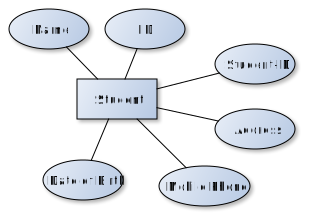
\includegraphics[width=0.45\linewidth]{\currentDir/../../../conceptualSchema/entitiesAndAttributes/yedErdEntitiesA21erd}}%
%
\floatSep%
%
\subfloat[][%
To start the \pgmodeler, under \ubuntu\ \linux, we open a \pgls{terminal} by hitting \ubuntuTerminal. %
We type in \bashil{pgmodler} and hit~\keys{\enter}. %
Under \microsoftWindows, you would instead proceed as shown in \cref{fig:installingPgModelerWindows22pgmodelerLogo}.%
\label{fig:makeStudentTable01startPgmodeler}%
]{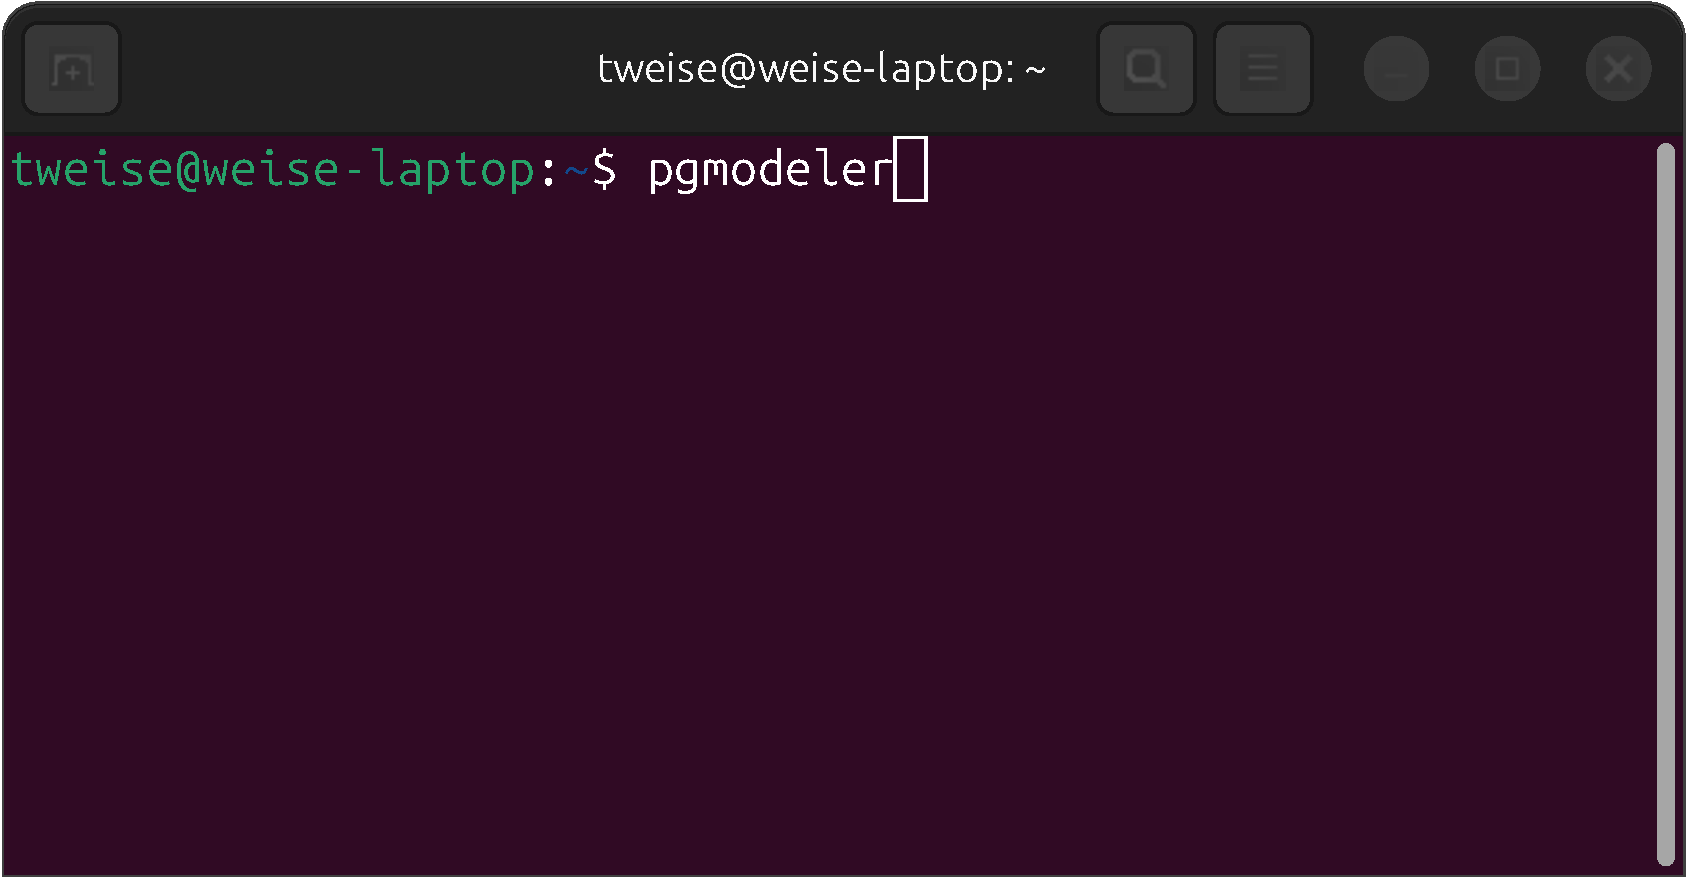
\includegraphics[width=0.53\linewidth]{\currentDir/makeStudentTable01startPgmodeler}}%
%
\floatRowSep%
%
\subfloat[][%
In the \pgmodeler, we click on \menu{New Model}.%
\label{fig:makeStudentTable02newModel}%
]{\tightbox{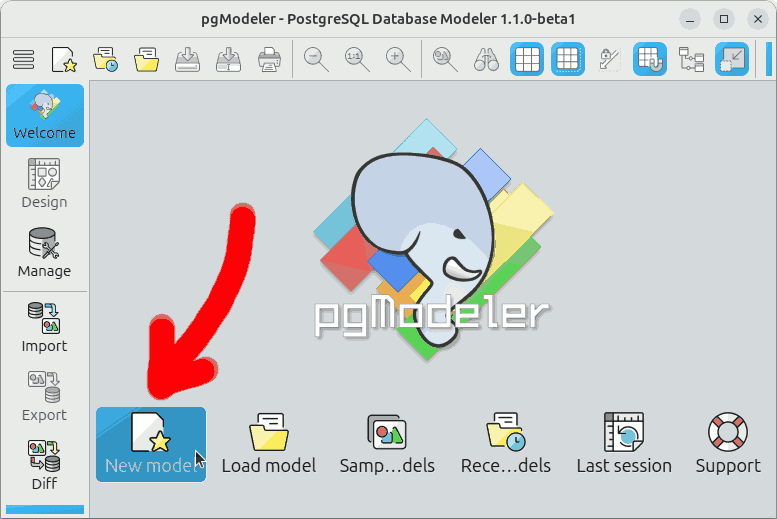
\includegraphics[width=0.48\linewidth]{\currentDir/makeStudentTable02newModel}}}%
%
\floatSep%
%
\subfloat[][%
An empty \pgls{ERD} opens. %
We right-click somewhere in it. %
In the context menu that opens, we click on \menu{Properties}.%
\label{fig:makeStudentTable03rightClickProperties}%
]{\tightbox{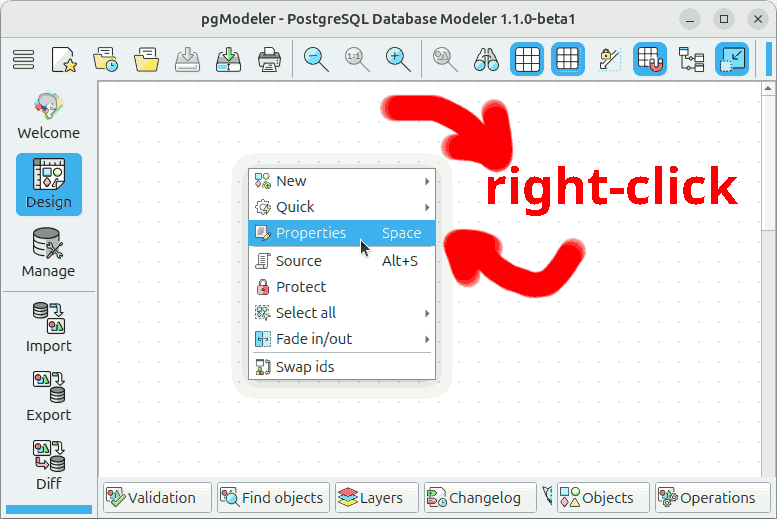
\includegraphics[width=0.48\linewidth]{\currentDir/makeStudentTable03rightClickProperties}}}%
%
\floatRowSep%
%
\subfloat[][%
A dialog called \inQuotes{Database Properties} opens. %
We want to set a proper name for our new \db. %
We choose \sqlil{student_database} and then click on~\menu{Apply}.%
\label{fig:makeStudentTable04propertiesNameApply}%
]{\tightbox{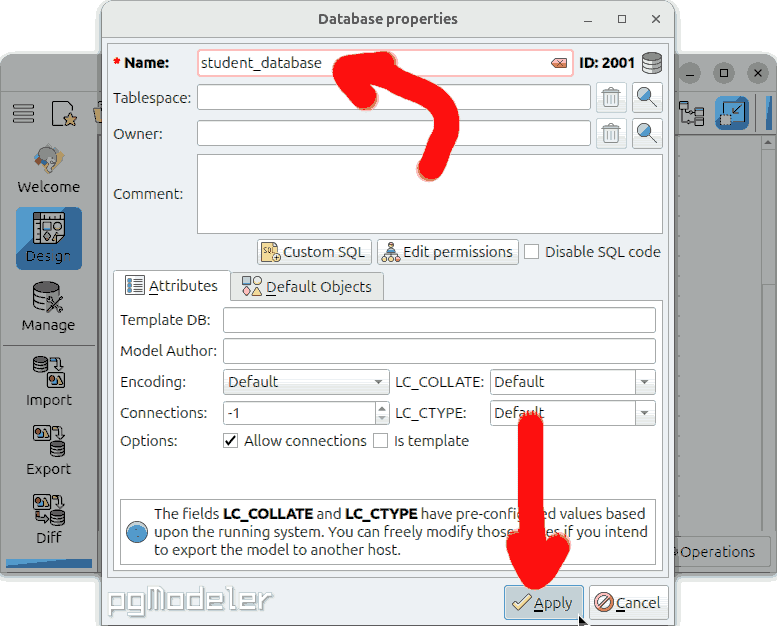
\includegraphics[width=0.48\linewidth]{\currentDir/makeStudentTable04propertiesNameApply}}}%
%
\floatSep%
%
\subfloat[][%
Back in the \pgls{ERD} view, we again right-click into the (empty) diagram. %
In the popup-menu, we click on~\menu{New>Schema Object>Table}.%
\label{fig:makeStudentTable05newTable}%
]{\tightbox{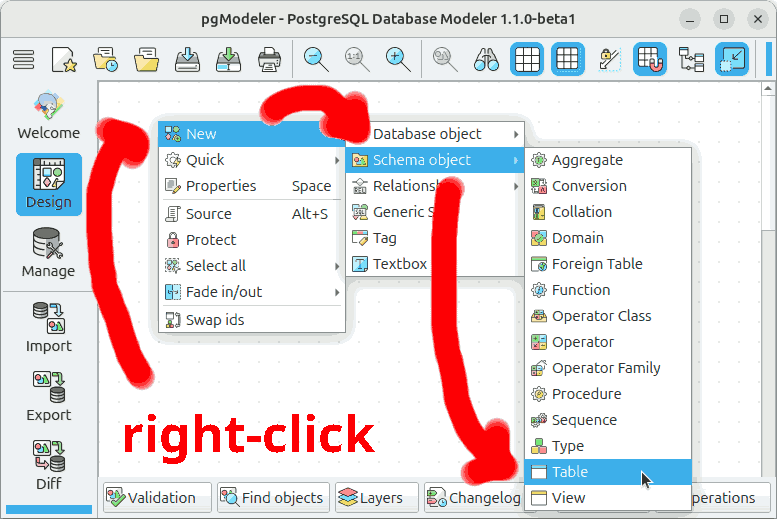
\includegraphics[width=0.48\linewidth]{\currentDir/makeStudentTable05newTable}}}%
%
\label{fig:makeStudentTable:A}%
\caption{Developing logical models using \pgmodeler.}%
\end{figure}%
%
\begin{figure}%
\ContinuedFloat%
\centering%
%
\subfloat[][%
The \inQuotes{Table properties} dialog opens. %
As table name, we enter \sqlil{student}. %
Then we click on the register~\menu{Columns}.%
\label{fig:makeStudentTable06tableNameColumns}%
]{\tightbox{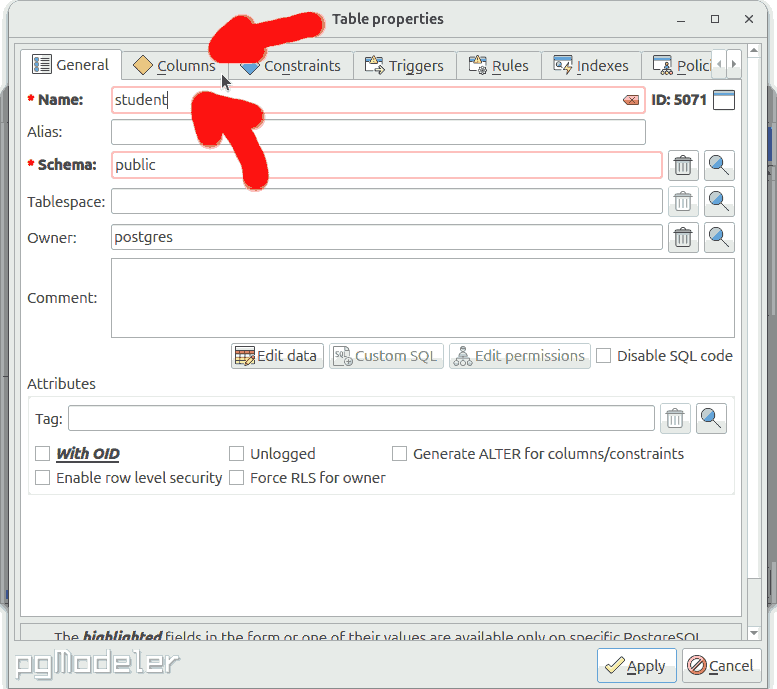
\includegraphics[width=0.48\linewidth]{\currentDir/makeStudentTable06tableNameColumns}}}%
%
\floatSep%
%
\subfloat[][%
In the columns register, we click on the \menu{Add Item} symbol~\pgmodelerAddItem.%
\label{fig:makeStudentTable07newColumn}%
]{\tightbox{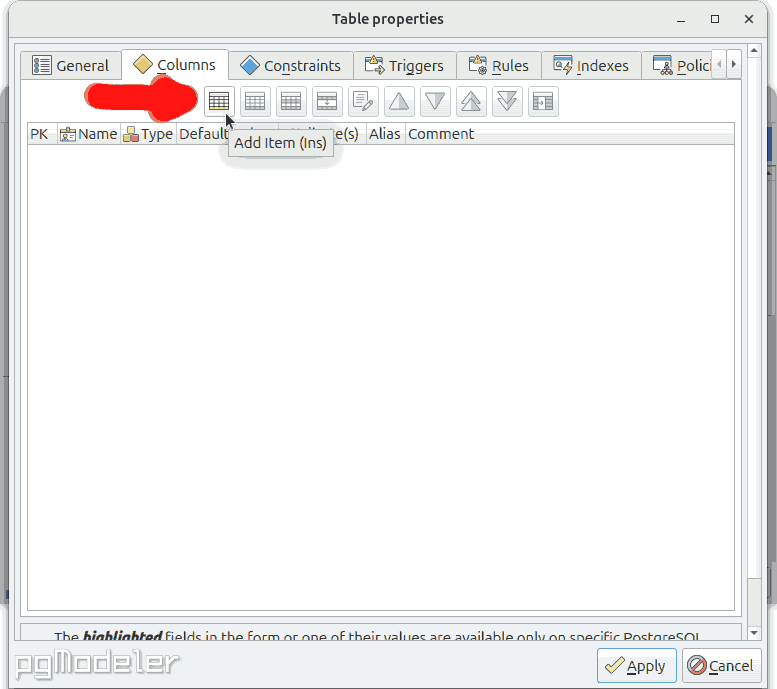
\includegraphics[width=0.48\linewidth]{\currentDir/makeStudentTable07newColumn}}}%
%
\floatRowSep%
%
\subfloat[][%
We want to add a column for the university-issued student~ID. %
As name for this column, we choose~\sqlil{student_id}. %
As type, we choose~\sqlil{character}\sqlIdx{CHARACTER}, i.e., the \sql\ datatype for fixed-length strings~(all student~IDs have the same length).%
\label{fig:makeStudentTable08studentIdNameAndType}%
]{\tightbox{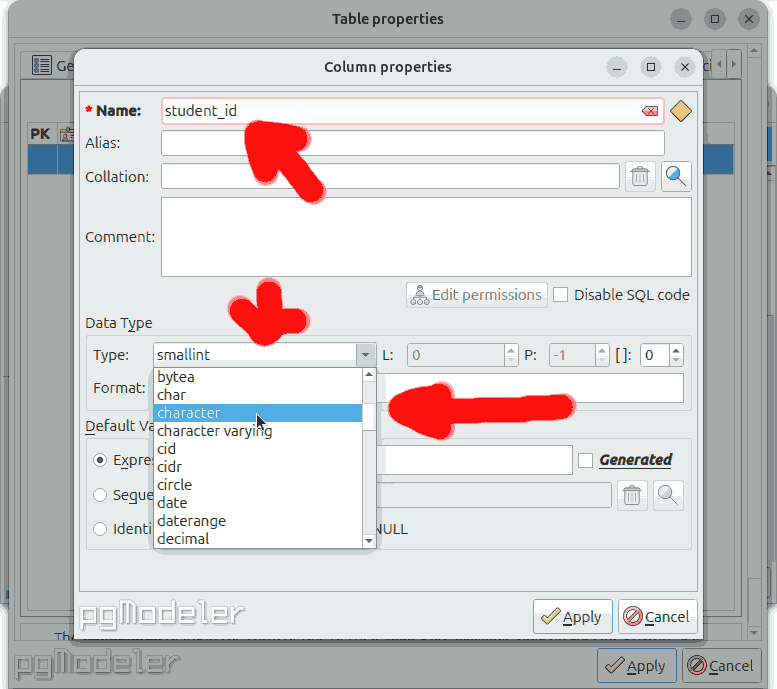
\includegraphics[width=0.48\linewidth]{\currentDir/makeStudentTable08studentIdNameAndType}}}%
%
\floatSep%
%
\subfloat[][%
As (fixed) length, we enter~11 in the \menu{L:}~field. %
We also mark the column as \sqlilIdx{NOT NULL}, meaning that there cannot be a student record without student~ID. %
We click~\menu{Apply}.%
\label{fig:makeStudentTable09studentIdLenNotNullApply}%
]{\tightbox{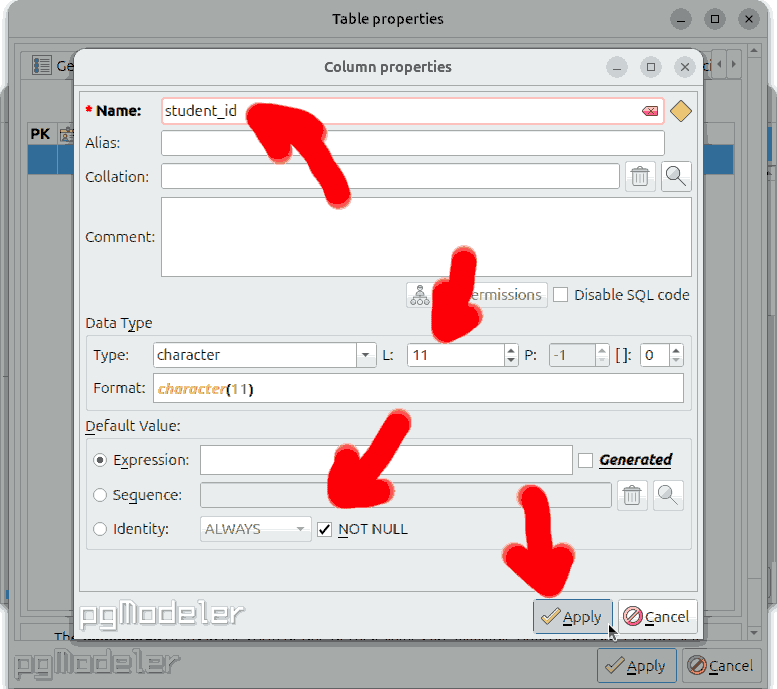
\includegraphics[width=0.48\linewidth]{\currentDir/makeStudentTable09studentIdLenNotNullApply}}}%
%
\label{fig:makeStudentTable:B}%
\caption{Developing logical models using \pgmodeler~(continued).}%
\end{figure}%
%
\begin{figure}%
\ContinuedFloat%
\centering%
%
\subfloat[][%
The new column appears in the dialog. %
We click again on~\menu{Add Item}~\pgmodelerAddItem.%
\label{fig:makeStudentTable10studentIdAddedNewColumn}%
]{\tightbox{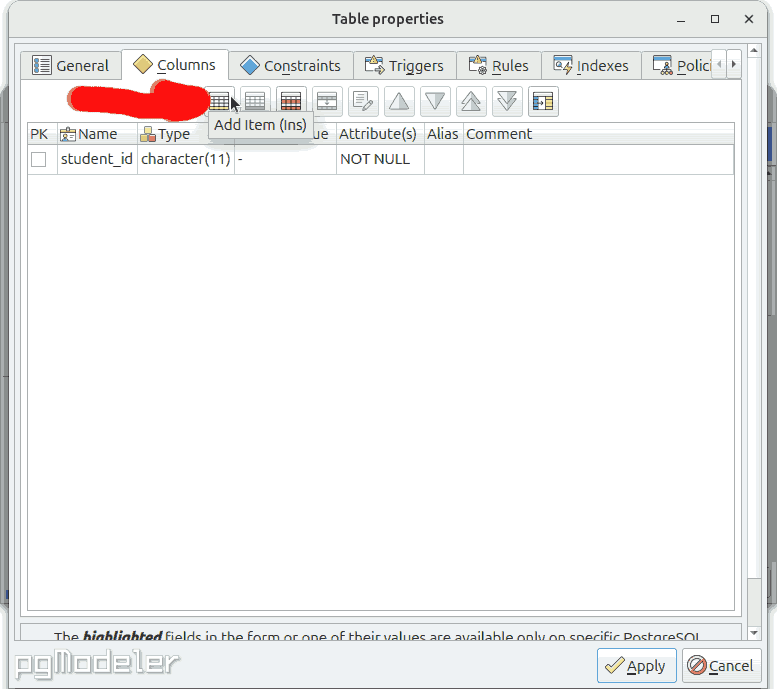
\includegraphics[width=0.48\linewidth]{\currentDir/makeStudentTable10studentIdAddedNewColumn}}}%
%
\floatSep%
%
\subfloat[][%
We add the column \sqlil{national_id} for storing Chinese~ID numbers~(中国公民身份号码). %
Such numbers are strings~(\sqlil{character}\sqlIdx{CHARACTER}) of the fixed length~18. %
We also mark this column as \sqlilIdx{NOT NULL}, meaning that every record must have one. %
We click~\menu{Apply}.%
\label{fig:makeStudentTable11nationalIdNameTypeLenNotNullApply}%
]{\tightbox{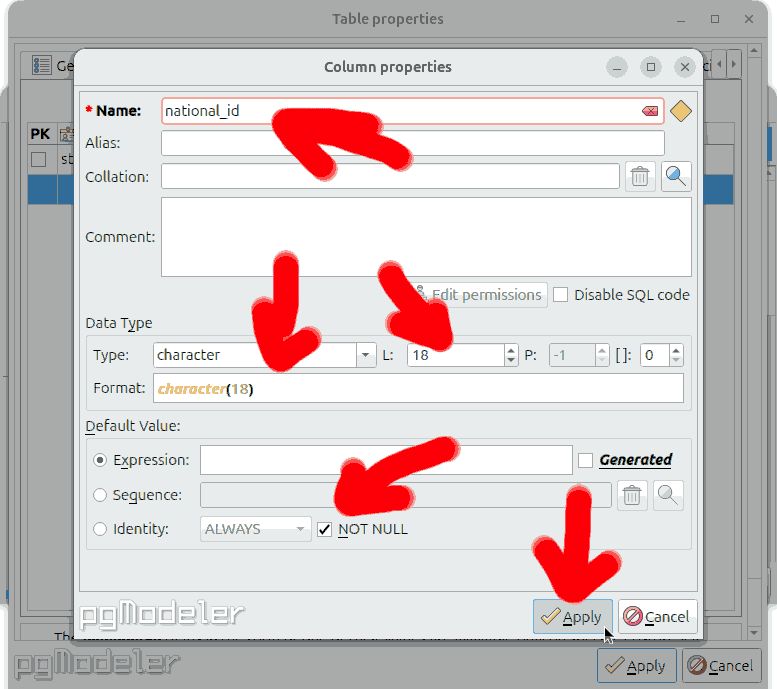
\includegraphics[width=0.48\linewidth]{\currentDir/makeStudentTable11nationalIdNameTypeLenNotNullApply}}}%
%
\floatRowSep%
%
\subfloat[][%
The new column appears and we click~\menu{Add Item}~\pgmodelerAddItem.%
\label{fig:makeStudentTable12nationalIdAddedNewColumn}%
]{\tightbox{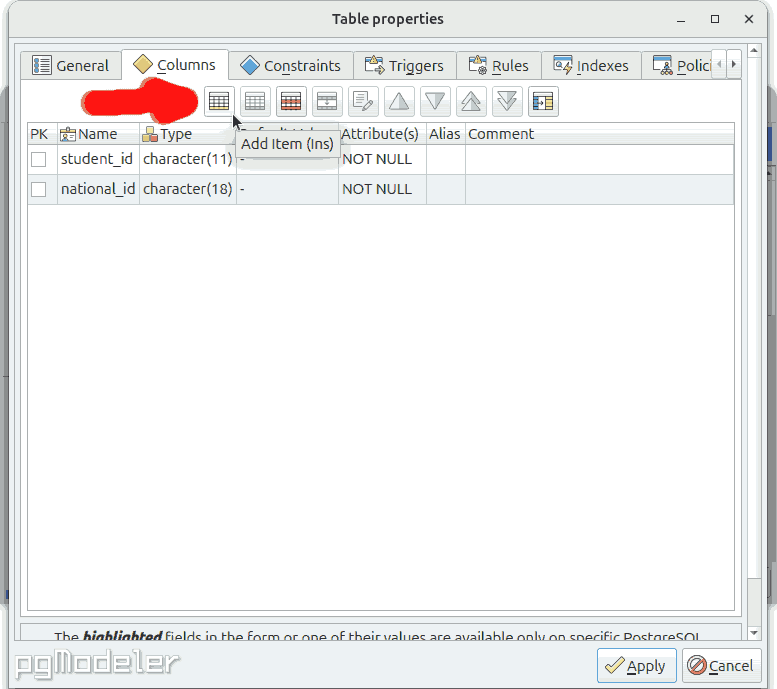
\includegraphics[width=0.48\linewidth]{\currentDir/makeStudentTable12nationalIdAddedNewColumn}}}%
%
\floatSep%
%
\subfloat[][%
We define the column \sqlil{name} for student names. %
Names are of variable length~(type \sqlil{varchar}\sqlIdx{VARCHAR}) and we set the \emph{maximum} length~255. %
Each student must have a name, so we again specify \sqlil{NOT NULL} and click~\menu{Apply}.%
\label{fig:makeStudentTable13nameNameTypeLenNotNullApply}%
]{\tightbox{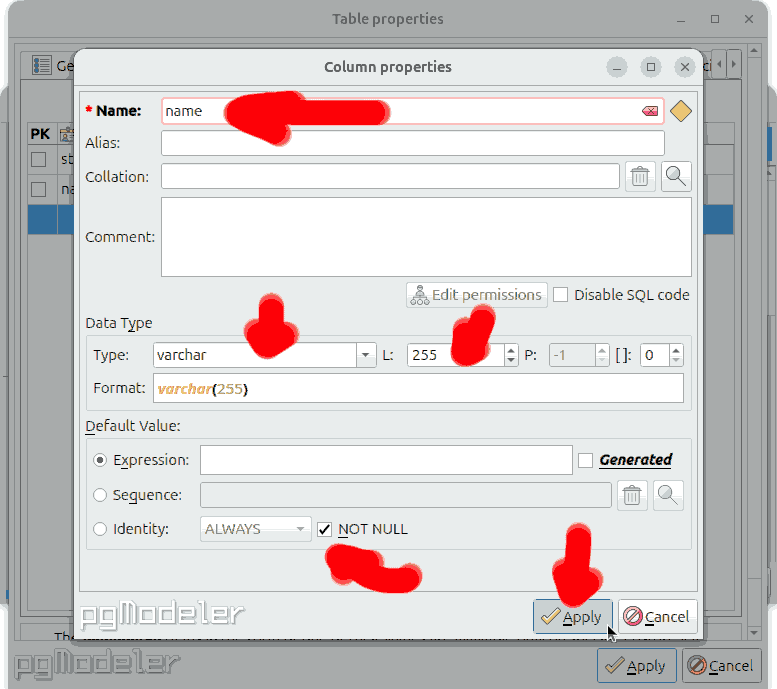
\includegraphics[width=0.48\linewidth]{\currentDir/makeStudentTable13nameNameTypeLenNotNullApply}}}%
%
\label{fig:makeStudentTable:C}%
\caption{Developing logical models using \pgmodeler~(continued).}%
\end{figure}%
%
\begin{figure}%
\ContinuedFloat%
\centering%
%
\subfloat[][%
The new column appears in the dialog. %
We click again on~\menu{Add Item}~\pgmodelerAddItem.%
\label{fig:makeStudentTable14nameAddedNewColumn}%
]{\tightbox{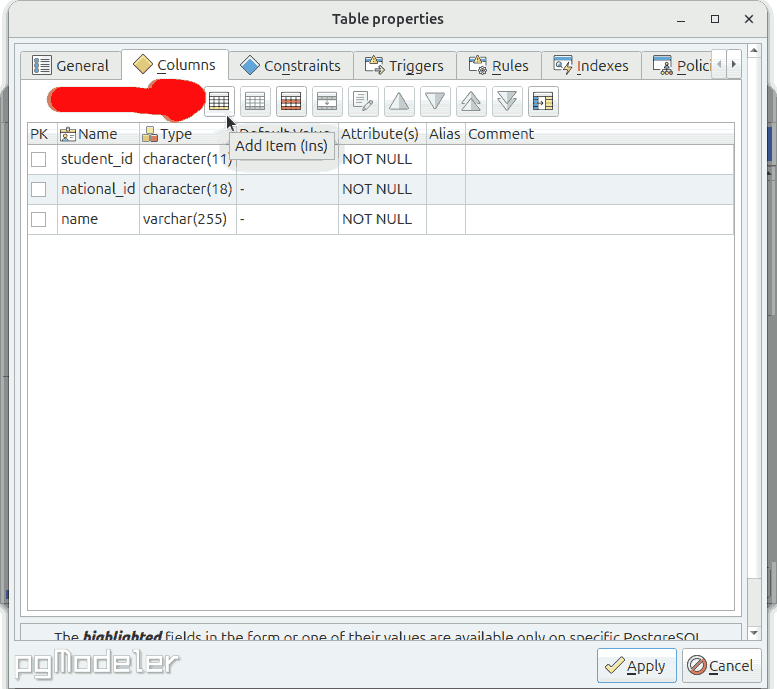
\includegraphics[width=0.48\linewidth]{\currentDir/makeStudentTable14nameAddedNewColumn}}}%
%
\floatSep%
%
\subfloat[][%
Addresses, too, are strings of variable length~(type \sqlil{varchar}\sqlIdx{VARCHAR}). %
We again set the maximum length to~255, require the field to be \sqlilIdx{NOT NULL}, and click~\menu{Apply}.%
\label{fig:makeStudentTable15addressNameTypeLenNotNullApply}%
]{\tightbox{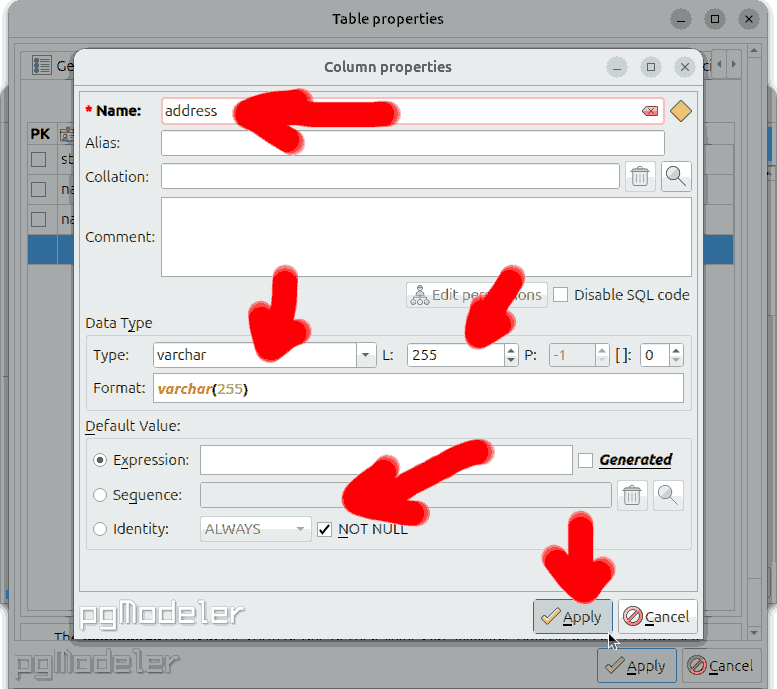
\includegraphics[width=0.48\linewidth]{\currentDir/makeStudentTable15addressNameTypeLenNotNullApply}}}%
%
\floatRowSep%
%
\subfloat[][%
The new column appears and we click~\menu{Add Item}~\pgmodelerAddItem.%
\label{fig:makeStudentTable16addressAddedNewColumn}%
]{\tightbox{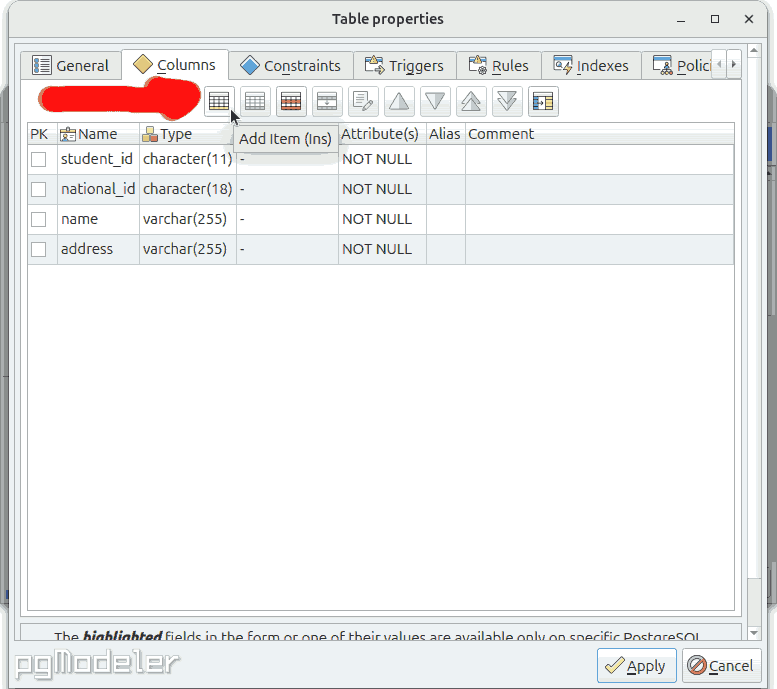
\includegraphics[width=0.48\linewidth]{\currentDir/makeStudentTable16addressAddedNewColumn}}}%
%
\floatSep%
%
\subfloat[][%
We now add a column for \sqlil{mobile} phone numbers. %
In China, these are strings~(\sqlil{character}\sqlIdx{CHARACTER}) of the fixed length~11. %
We require that they must be specified~(\sqlilIdx{NOT NULL}) and click~\menu{Apply}.%
\label{fig:makeStudentTable17mobileNameTypeLenNotNullApply}%
]{\tightbox{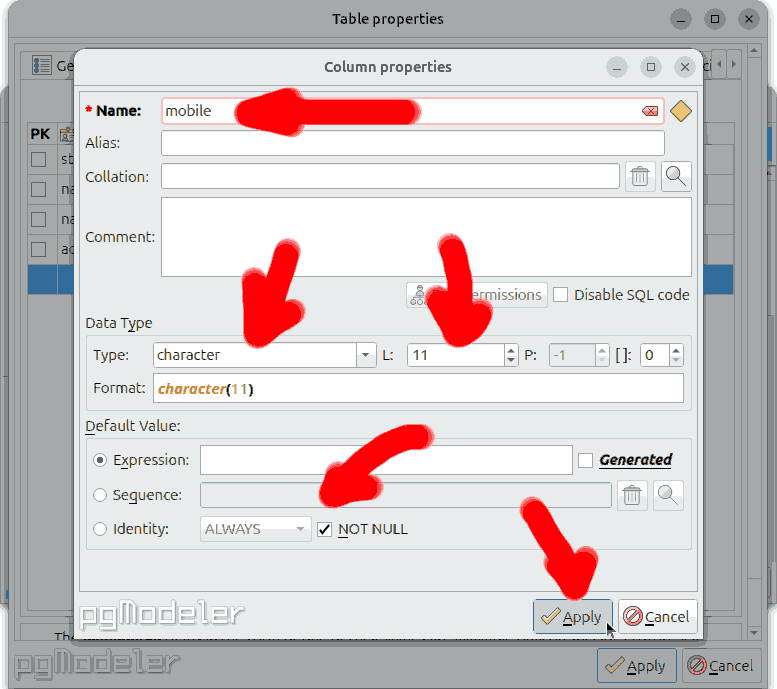
\includegraphics[width=0.48\linewidth]{\currentDir/makeStudentTable17mobileNameTypeLenNotNullApply}}}%
%
\label{fig:makeStudentTable:D}%
\caption{Developing logical models using \pgmodeler~(continued).}%
\end{figure}%
%
\begin{figure}%
\ContinuedFloat%
\centering%
%
\subfloat[][%
The new column appears in the dialog. %
We click again on~\menu{Add Item}~\pgmodelerAddItem.%
\label{fig:makeStudentTable18mobileAddedNewColumn}%
]{\tightbox{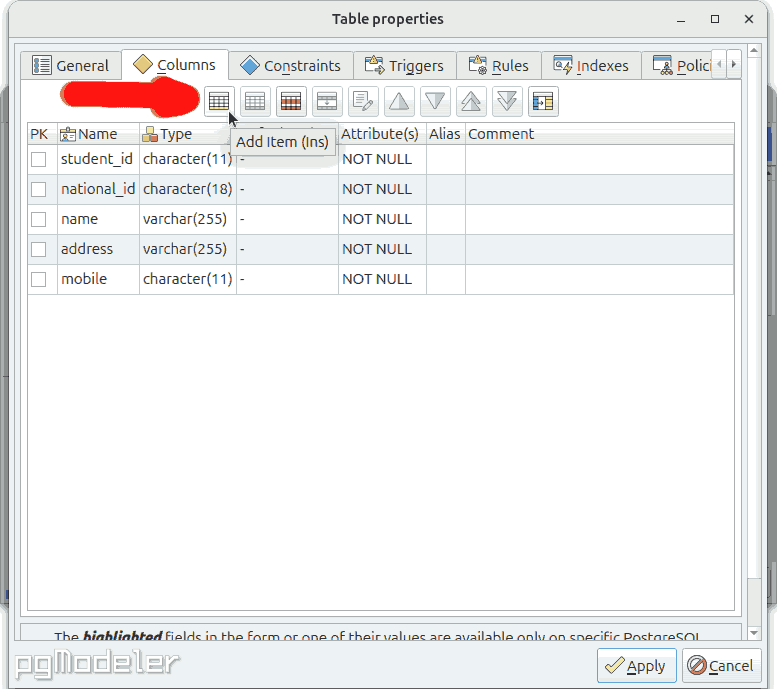
\includegraphics[width=0.48\linewidth]{\currentDir/makeStudentTable18mobileAddedNewColumn}}}%
%
\floatSep%
%
\subfloat[][%
Finally, we add the \glsreset{dateOfBirth}\pgls{dateOfBirth} in form of a \sqlil{date_of_birth} column. %
The type here is \sqlil{date}\sqlIdx{DATE} and \pglspl{dateOfBirth} are required to be \sqlilIdx{NOT NULL}. %
We click~\menu{Apply}.%
\label{fig:makeStudentTable19dateOfBirthNameTypeNotNullApply}%
]{\tightbox{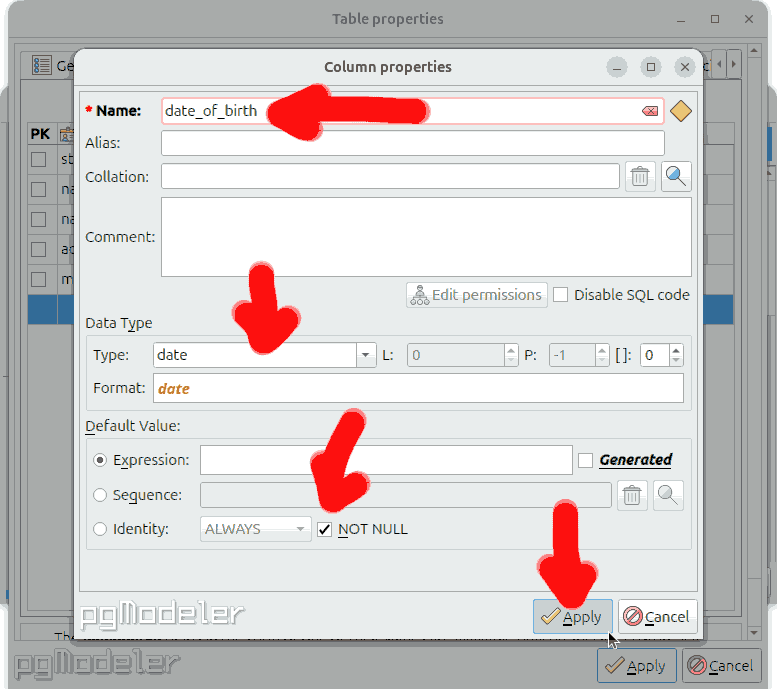
\includegraphics[width=0.48\linewidth]{\currentDir/makeStudentTable19dateOfBirthNameTypeNotNullApply}}}%
%
\floatRowSep%
%
\subfloat[][%
The new column appears. %
We click on the register \menu{Constraints}, because now we want to add validity rules for our data.%
\label{fig:makeStudentTable20dateOfBirthAddedConstraints}%
]{\tightbox{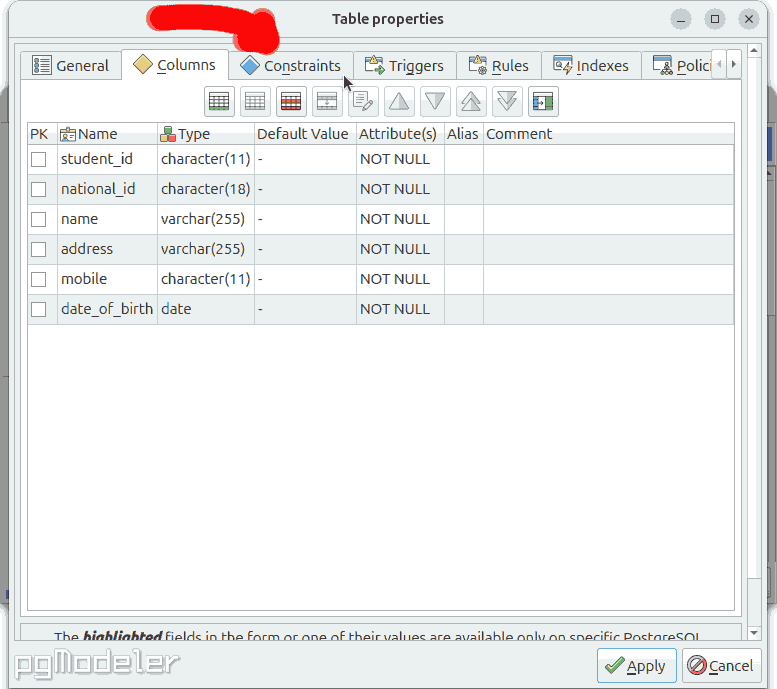
\includegraphics[width=0.48\linewidth]{\currentDir/makeStudentTable20dateOfBirthAddedConstraints}}}%
%
\floatSep%
%
\subfloat[][%
In the \menu{Constraints} register, we click~\menu{Add Item}~\pgmodelerAddItem.%
\label{fig:makeStudentTable21newConstraint}%
]{\tightbox{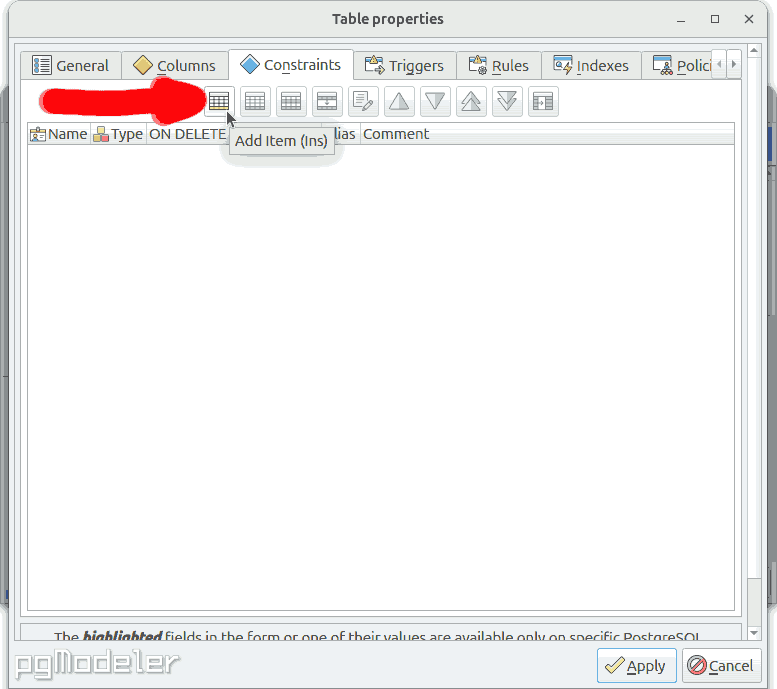
\includegraphics[width=0.48\linewidth]{\currentDir/makeStudentTable21newConstraint}}}%
%
\label{fig:makeStudentTable:E}%
\caption{Developing logical models using \pgmodeler~(continued).}%
\end{figure}%
%
\begin{figure}%
\ContinuedFloat%
\centering%
%
\subfloat[][%
As first constraint, we want to define \sqlil{student_id} as the primary key of our table. %
We call this constraint \sqlil{student_student_id_pk} and select \sqlilIdx{PRIMARY KEY} as type. %
We select the column \sqlil{student_id} in the \menu{Column} drop-down box and click on~\menu{Add Item}~\pgmodelerAddItem.%
\label{fig:makeStudentTable22studentIdPkData}%
]{\tightbox{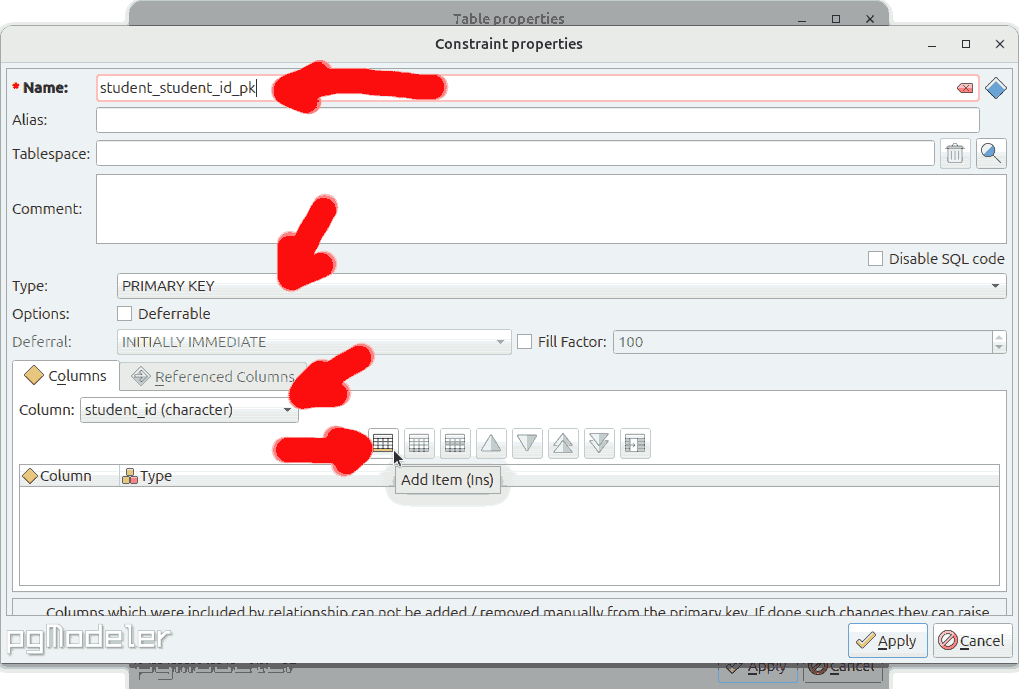
\includegraphics[width=0.48\linewidth]{\currentDir/makeStudentTable22studentIdPkData}}}%
%
\floatSep%
%
\subfloat[][%
The column \sqlil{student_id} appears in the \menu{Columns} list. %
We click on~\menu{Apply}.%
\label{fig:makeStudentTable23studentIdColAddedApply}%
]{\tightbox{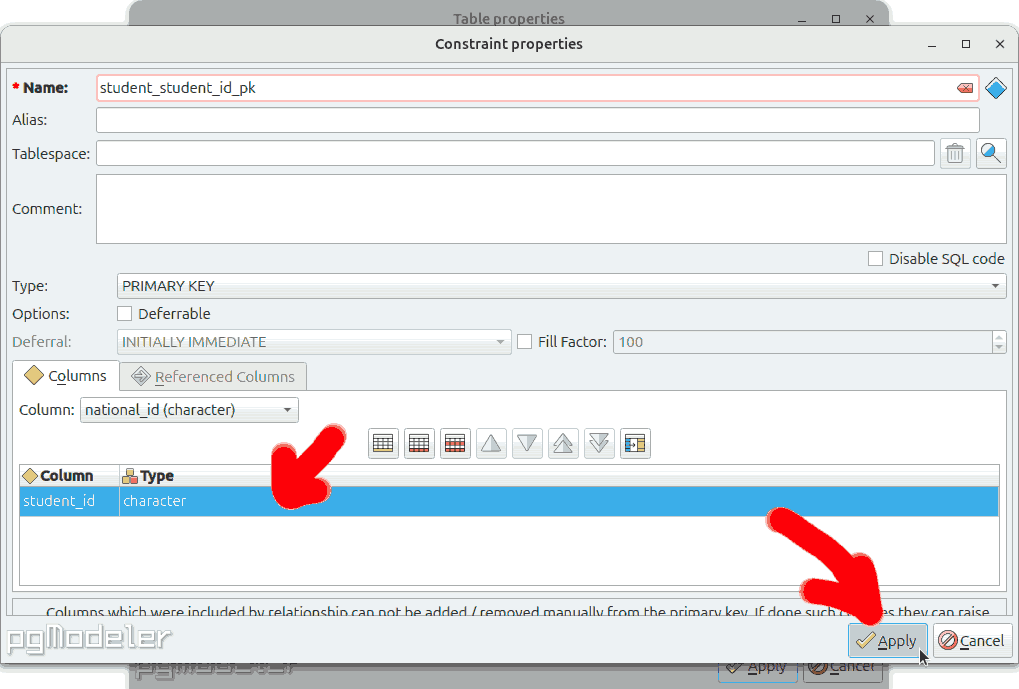
\includegraphics[width=0.48\linewidth]{\currentDir/makeStudentTable23studentIdColAddedApply}}}%
%
\floatRowSep%
%
\subfloat[][%
The new constraint appears and we click on \menu{Add Item}~\pgmodelerAddItem.%
\label{fig:makeStudentTable24studentIdAddedNewConstraint}%
]{\tightbox{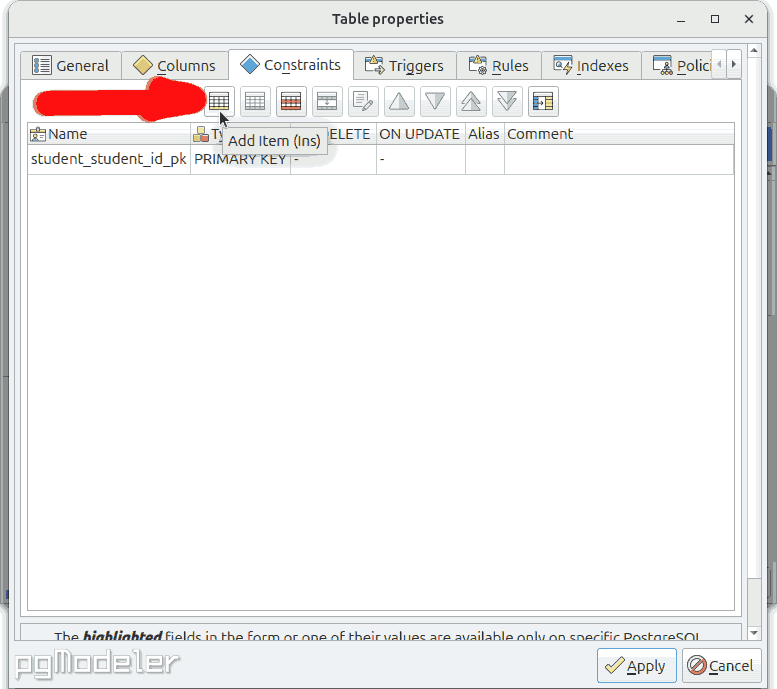
\includegraphics[width=0.48\linewidth]{\currentDir/makeStudentTable24studentIdAddedNewConstraint}}}%
%
\floatSep%
%
\subfloat[][%
We now want to add a constraint checking that the national~ID is correct. %
We call it \sqlil{student_national_id_check} and select \sqlil{CHECK}\sqlIdx{CONSTRAINT!CHECK} in the \menu{Type} drop-down box.
\label{fig:makeStudentTable25nationalIdCheck}%
]{\tightbox{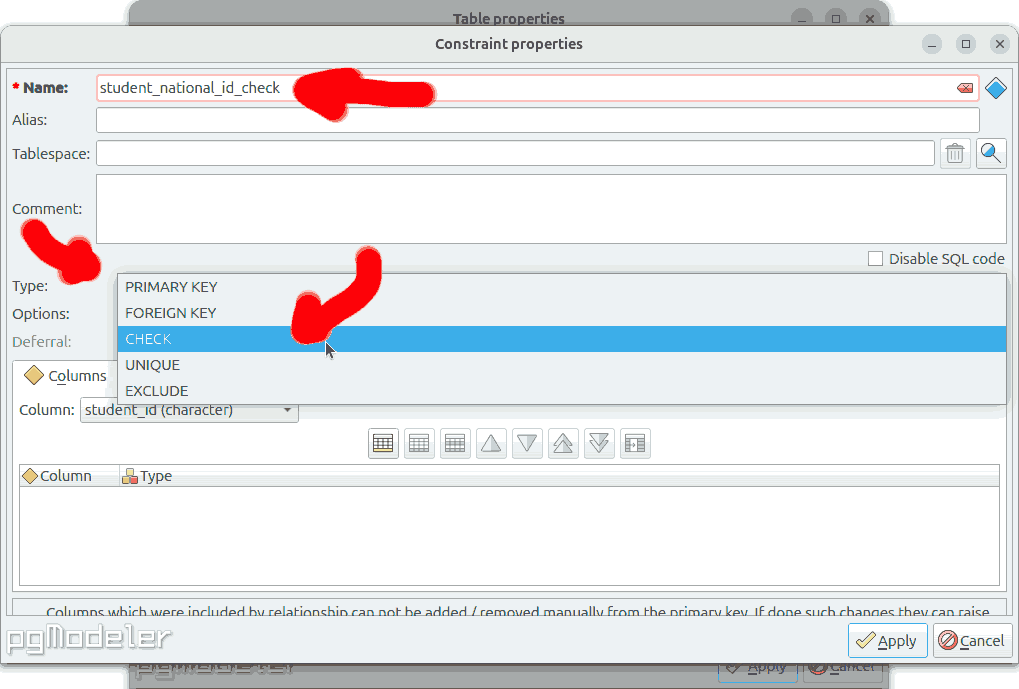
\includegraphics[width=0.48\linewidth]{\currentDir/makeStudentTable25nationalIdCheck}}}%
%
\label{fig:makeStudentTable:F}%
\caption{Developing logical models using \pgmodeler~(continued).}%
\end{figure}%
%
\begin{figure}%
\ContinuedFloat%
\centering%
%
\subfloat[][{\sloppy%
\sqlil{CHECK}\sqlIdx{CONSTRAINT!CHECK} constraints are specified as \sql\ \menu{Expression}. %
To validate the field~\sqlil{national_id}, we specify the \pgls{regex} \sqlil{national_id~'^\\d\{6\}((19)|(20))\\d\{9\}[0-9X]\$'}. %
We click~\menu{Apply}.}%
\label{fig:makeStudentTable26nationalIdConstraintApply}%
]{\tightbox{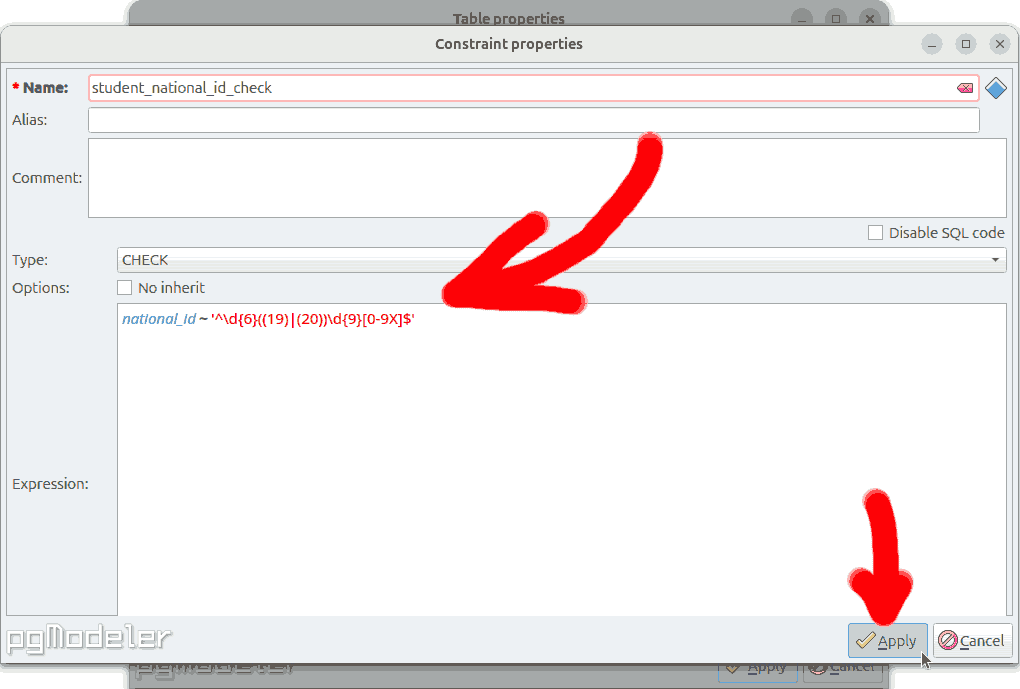
\includegraphics[width=0.48\linewidth]{\currentDir/makeStudentTable26nationalIdConstraintApply}}}%
%
\floatSep%
%
\subfloat[][%
The new constraint appears and we click on~\menu{Add Item}~\pgmodelerAddItem.%
\label{fig:makeStudentTable27nationalIdAddedNewConstraint}%
]{\tightbox{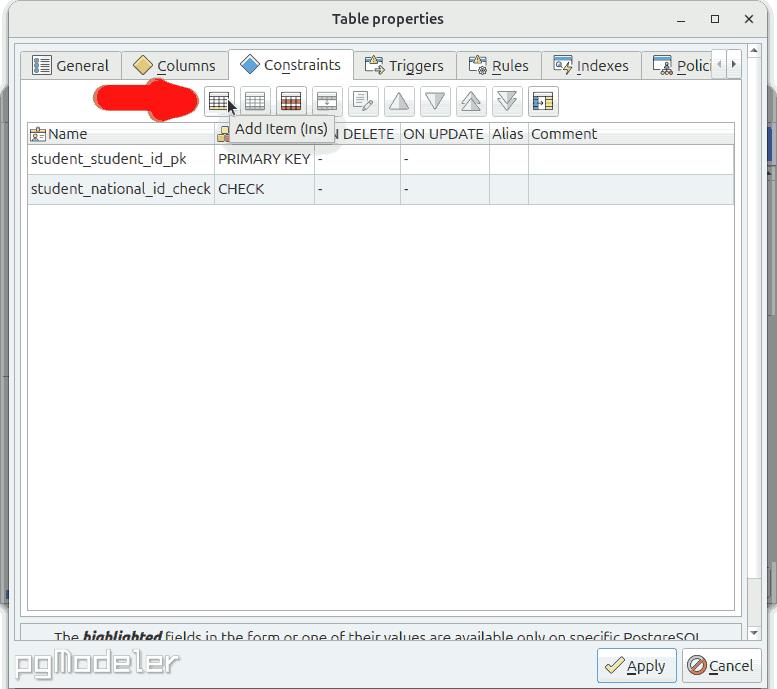
\includegraphics[width=0.48\linewidth]{\currentDir/makeStudentTable27nationalIdAddedNewConstraint}}}%
%
\floatRowSep%
%
\subfloat[][%
We create a \sqlil{CHECK}\sqlIdx{CONSTRAINT!CHECK}~constraint for the column~\sqlil{mobile}. %
The expression~\sqlil{mobile ~ '^\\d\{11\}\$'} demands an 11~digit string. %
We click on~\menu{Apply}.%
\label{fig:makeStudentTable28mobileCheck}%
]{\tightbox{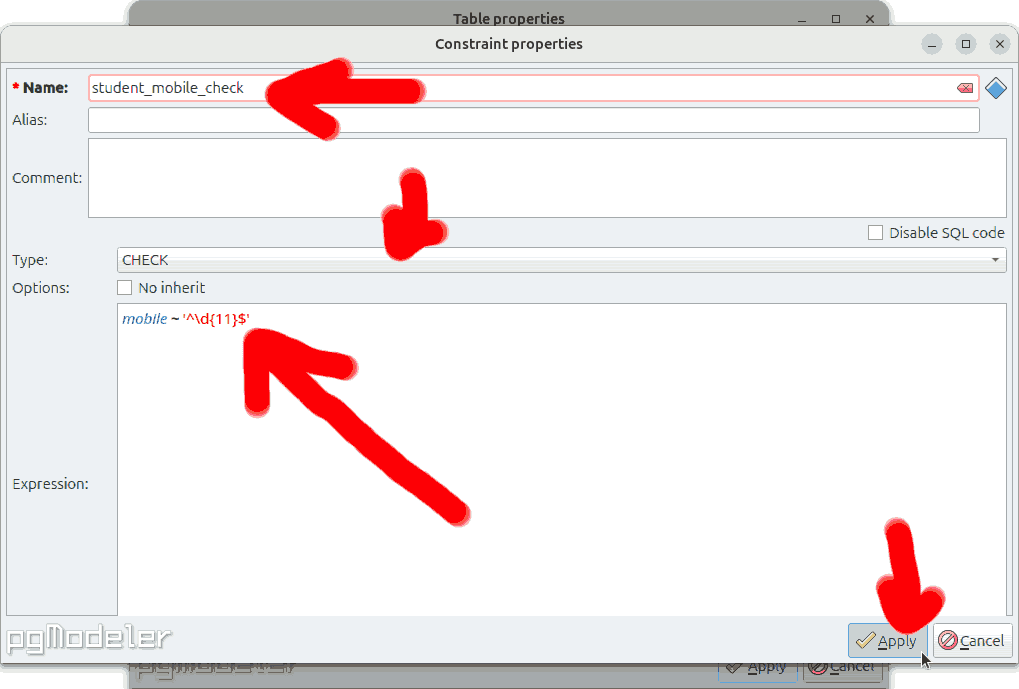
\includegraphics[width=0.48\linewidth]{\currentDir/makeStudentTable28mobileCheck}}}%
%
\floatSep%
%
\subfloat[][%
The new constraint appears and we click on~\menu{Add Item}~\pgmodelerAddItem.%
\label{fig:makeStudentTable29mobileAddedNewConstraint}%
]{\tightbox{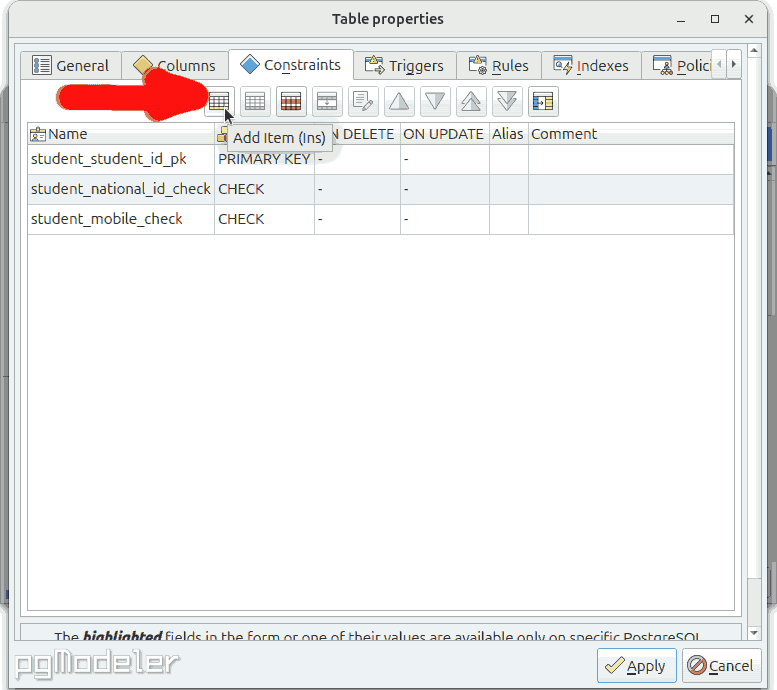
\includegraphics[width=0.48\linewidth]{\currentDir/makeStudentTable29mobileAddedNewConstraint}}}%
%
\label{fig:makeStudentTable:G}%
\caption{Developing logical models using \pgmodeler~(continued).}%
\end{figure}%
%
\begin{figure}%
\ContinuedFloat%
\centering%
%
\subfloat[][%
We specify the \sqlil{CHECK}\sqlIdx{CONSTRAINT!CHECK} constraint for the \pgls{dateOfBirth} and call it~\sqlil{student_date_of_birth_check}. %
We combine the condition \sqlil{date_of_birth > '1900-01-01'} (demanding that students may not be born before the year~1900) and \sqlil{date_of_birth < '2100-01-01'}~(which prevents students born in the 22nd century) with~\sqlilIdx{AND}. %
We click~\menu{Apply}.%
\label{fig:makeStudentTable30dateOfBirthCheck}%
]{\tightbox{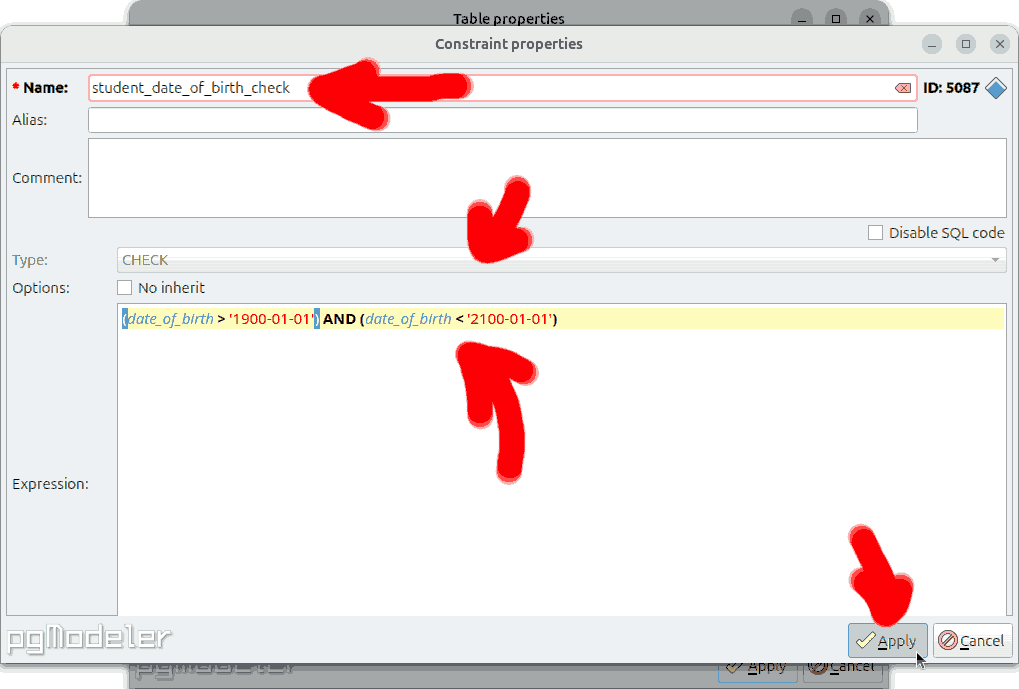
\includegraphics[width=0.48\linewidth]{\currentDir/makeStudentTable30dateOfBirthCheck}}}%
%
\floatSep%
%
\subfloat[][%
The new constraint appears and we click on~\menu{Add Item}~\pgmodelerAddItem.%
\label{fig:makeStudentTable31dateOfBirthAddedNewConstraint}%
]{\tightbox{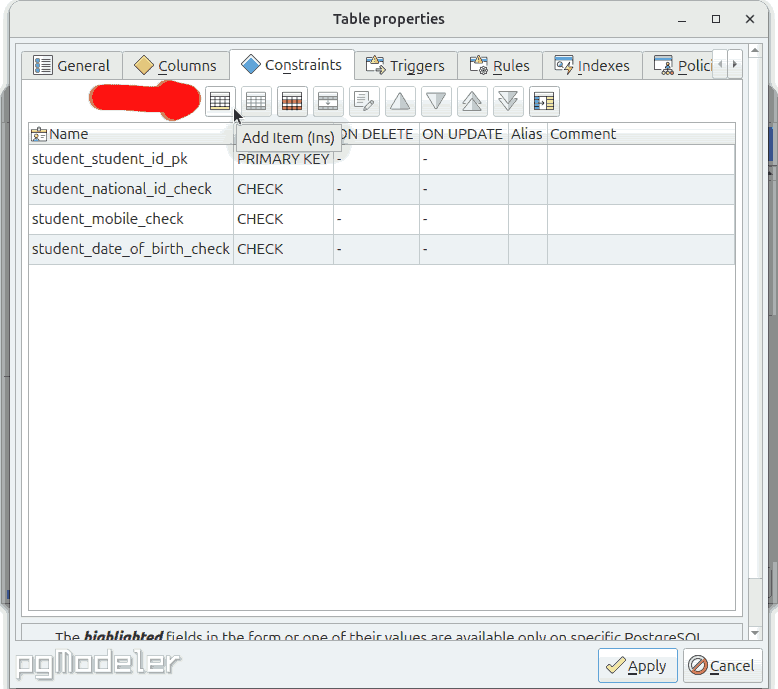
\includegraphics[width=0.48\linewidth]{\currentDir/makeStudentTable31dateOfBirthAddedNewConstraint}}}%
%
\floatRowSep%
%
\subfloat[][%
We create a \sqlil{CHECK}\sqlIdx{CONSTRAINT!CHECK}~constraint for the column~\sqlil{name} and call it~\sqlil{student_name_check}. %
The expression~\expandafter\sqlil{name ~ '^\\S+.*\\S+\$'} demands that names both start and end with printable characters and may contain an arbitrary number of characters in between %
We click on~\menu{Apply}.%
\label{fig:makeStudentTable32nameCheck}%
]{\tightbox{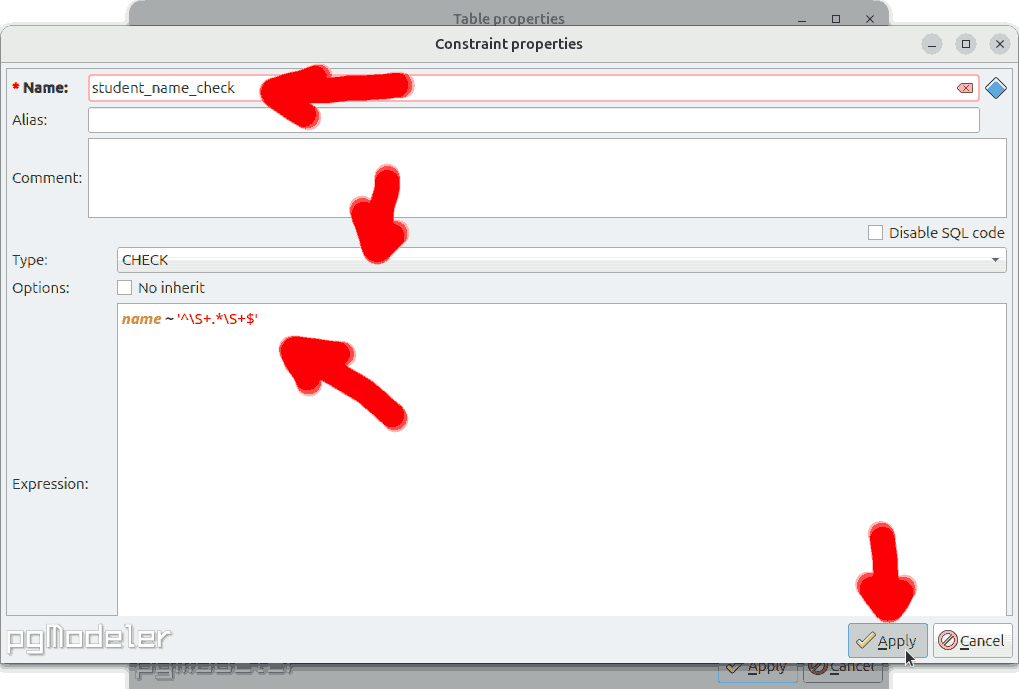
\includegraphics[width=0.48\linewidth]{\currentDir/makeStudentTable32nameCheck}}}%
%
\floatSep%
%
\subfloat[][%
The new constraint appears. %
We stop here and create the table model by clicking on~\menu{Apply}.%
\label{fig:makeStudentTable33nameCheckAddedApply}%
]{\tightbox{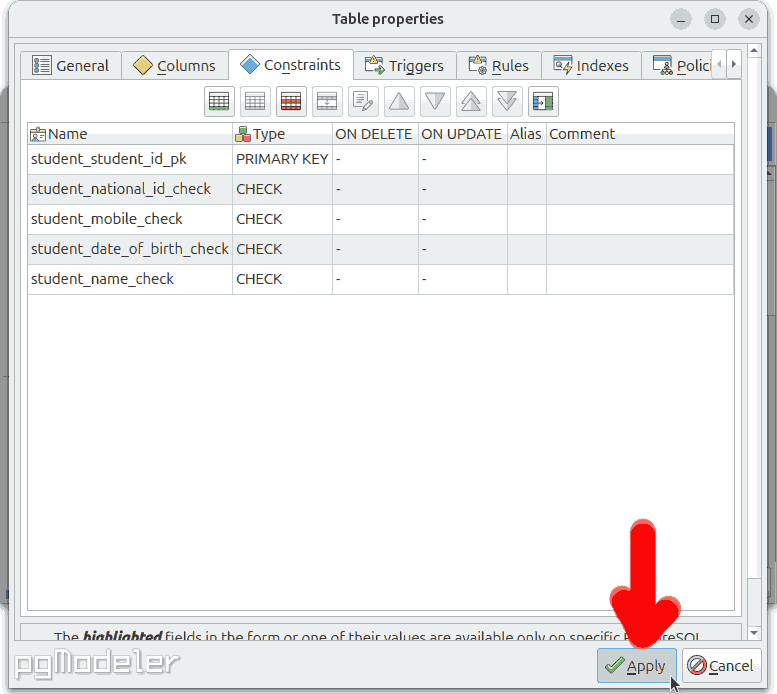
\includegraphics[width=0.48\linewidth]{\currentDir/makeStudentTable33nameCheckAddedApply}}}%
%
\label{fig:makeStudentTable:H}%
\caption{Developing logical models using \pgmodeler~(continued).}%
\end{figure}%
%
\begin{figure}%
\ContinuedFloat%
\centering%
%
\subfloat[][%
The new table appears in our \pgls{ERD}, with a syntax similar to what we had in \cref{sec:compactCrowsFootNotation}. %
We click on the main menu~\pgmodelerMainMenu.
\label{fig:makeStudentTable34modelMenu}%
]{\tightbox{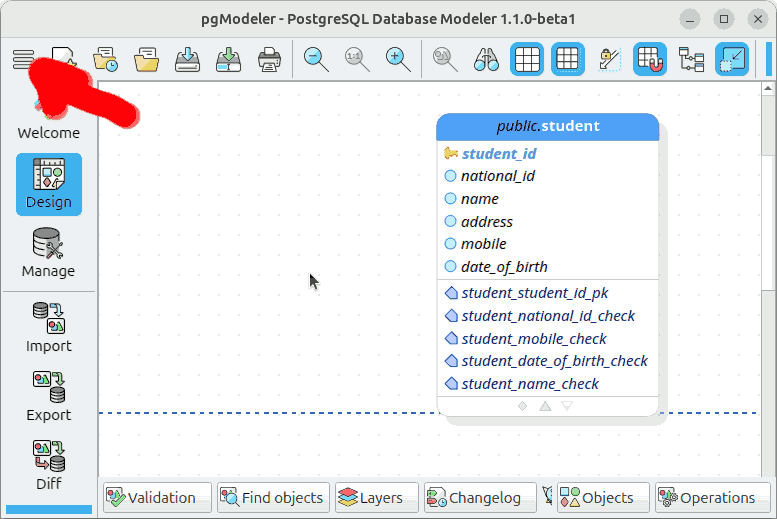
\includegraphics[width=0.48\linewidth]{\currentDir/makeStudentTable34modelMenu}}}%
%
\floatSep%
%
\subfloat[][%
It is time to save the model to a file. %
We click on~\menu{\pgmodelerMainMenu>File>Save as}.
\label{fig:makeStudentTable35saveAs}%
]{\tightbox{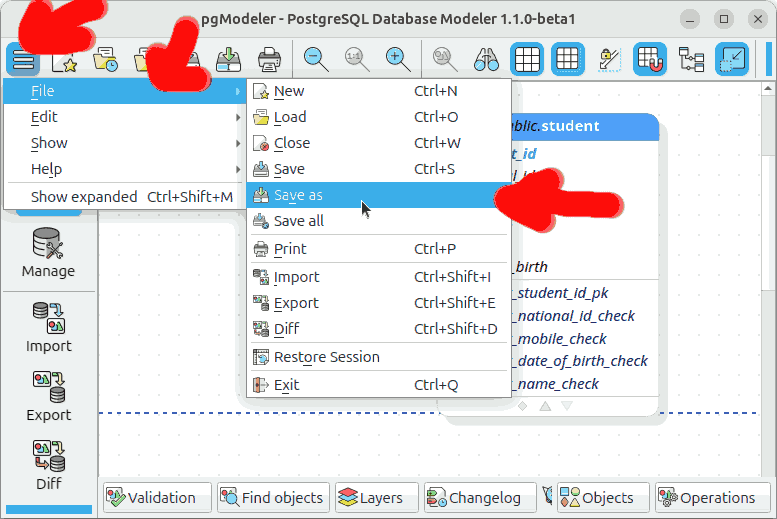
\includegraphics[width=0.48\linewidth]{\currentDir/makeStudentTable35saveAs}}}%
%
\floatRowSep%
%
\subfloat[][%
Since our model is new and unchecked (or changed), we get asked to validate it. %
Heck, why not, we click on~\menu{Validate}.%
\label{fig:makeStudentTable36shouldValidate}%
]{\tightbox{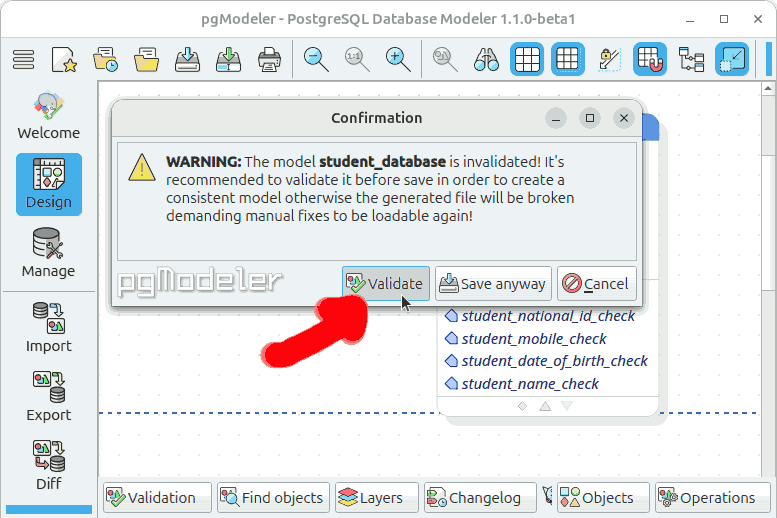
\includegraphics[width=0.48\linewidth]{\currentDir/makeStudentTable36shouldValidate}}}%
%
\floatSep%
%
\subfloat[][%
We can now select a file name and directory where the model should be stored. %
We choose the name \sqlil{student_database} and click~\menu{Save}.%
\label{fig:makeStudentTable37saveAsWhere}%
]{\tightbox{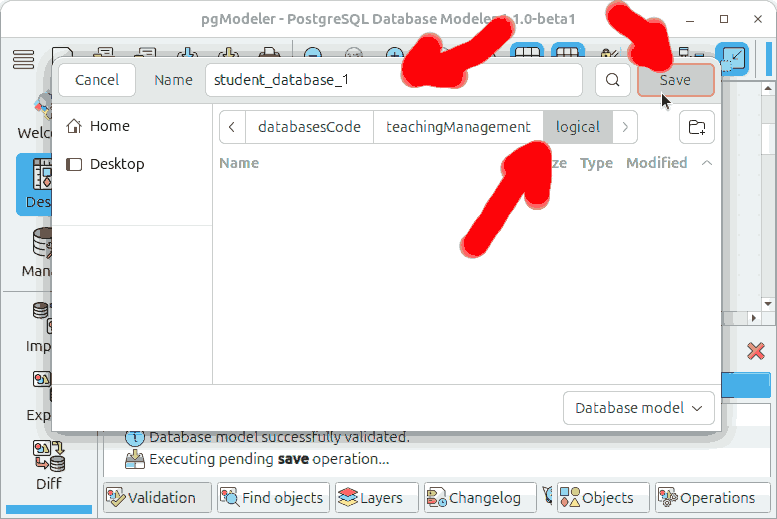
\includegraphics[width=0.48\linewidth]{\currentDir/makeStudentTable37saveAsWhere}}}%
%
\label{fig:makeStudentTable:I}%
\caption{Developing logical models using \pgmodeler~(continued).}%
\end{figure}%
%
\begin{figure}%
\ContinuedFloat%
\centering%
%
\subfloat[][%
This takes us back to the main window. %
We notice a bar with new buttons, including one called~\menu{Validate}. %
We click on it.%
\label{fig:makeStudentTable38validate}%
]{\tightbox{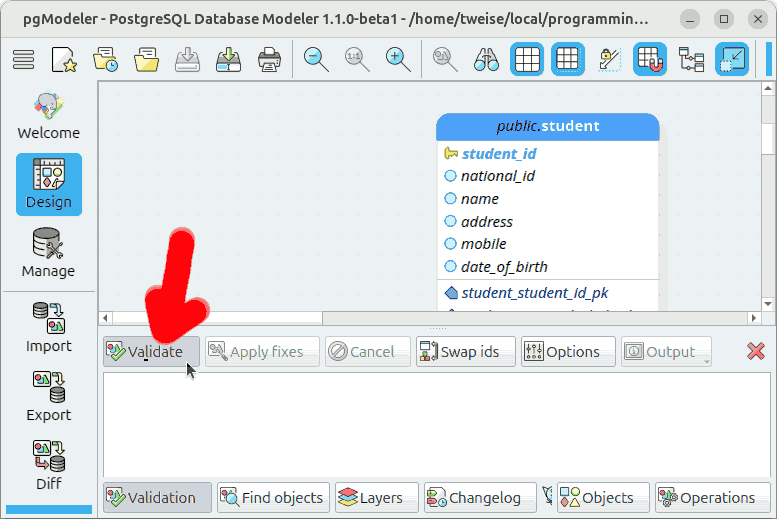
\includegraphics[width=0.48\linewidth]{\currentDir/makeStudentTable38validate}}}%
%
\floatSep%
%
\subfloat[][%
Our model gets validated. %
It is OK. %
We can close the log.%
\label{fig:makeStudentTable39validated}%
]{\tightbox{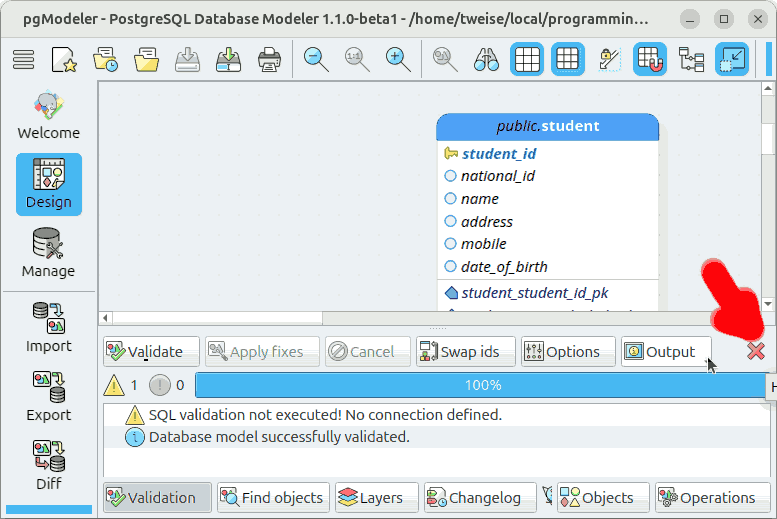
\includegraphics[width=0.48\linewidth]{\currentDir/makeStudentTable39validated}}}%
%
\floatRowSep%
%
\subfloat[][%
We now want to export the model and, thus, click on~\menu{Export}.%
\label{fig:makeStudentTable40export}%
]{\tightbox{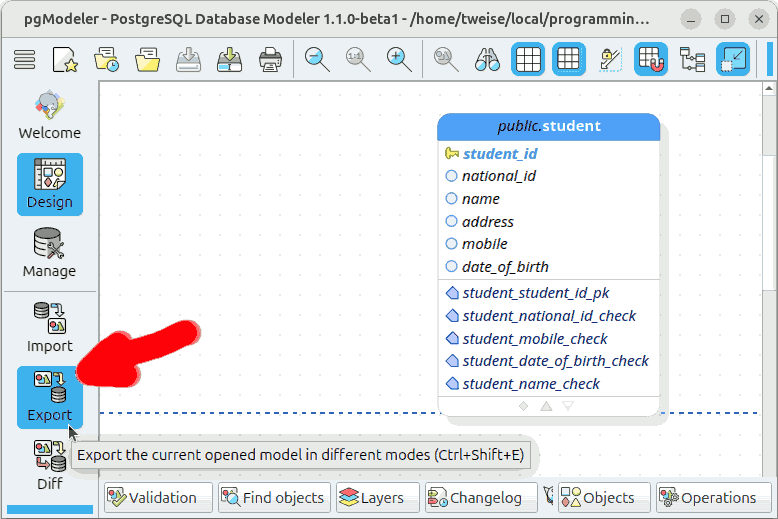
\includegraphics[width=0.48\linewidth]{\currentDir/makeStudentTable40export}}}%
%
\floatSep%
%
\subfloat[][%
We want to store it as graphic. %
So we click on \menu{Graphics file} and select \menu{Vectorial~(SVG)}, which will store the model in \pgls{SVG}~format. %
We then click into the \menu{File}~bar.
\label{fig:makeStudentTable41exportAsSvg}%
]{\tightbox{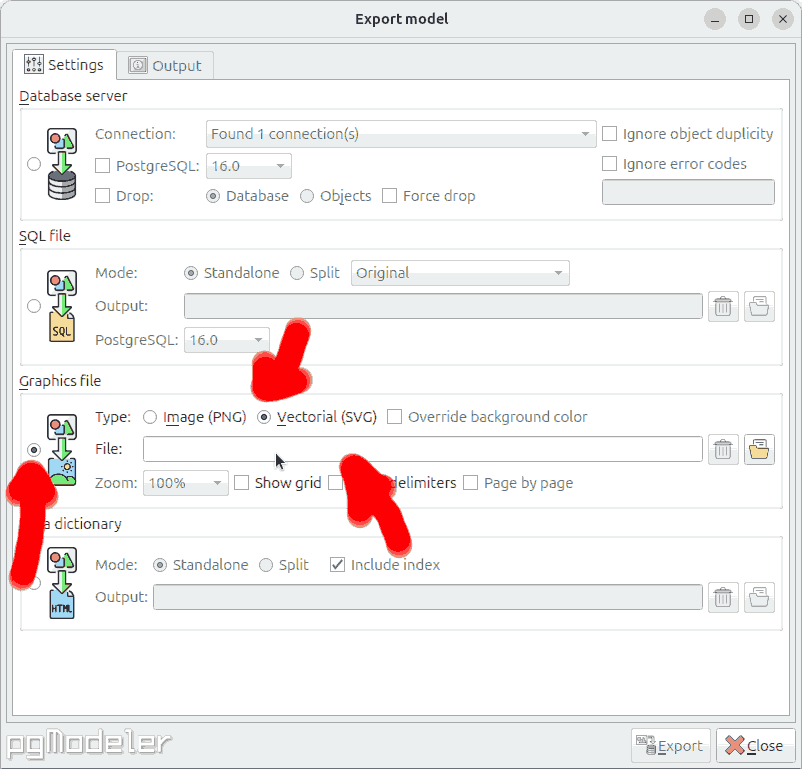
\includegraphics[width=0.48\linewidth]{\currentDir/makeStudentTable41exportAsSvg}}}%
%
\label{fig:makeStudentTable:J}%
\caption{Developing logical models using \pgmodeler~(continued).}%
\end{figure}%
%
\begin{figure}%
\ContinuedFloat%
\centering%
%
\subfloat[][%
We again get to select a file name and stick with \sqlil{student_database}. %
We click on~\menu{Save}.%
\label{fig:makeStudentTable42fileName}%
]{\tightbox{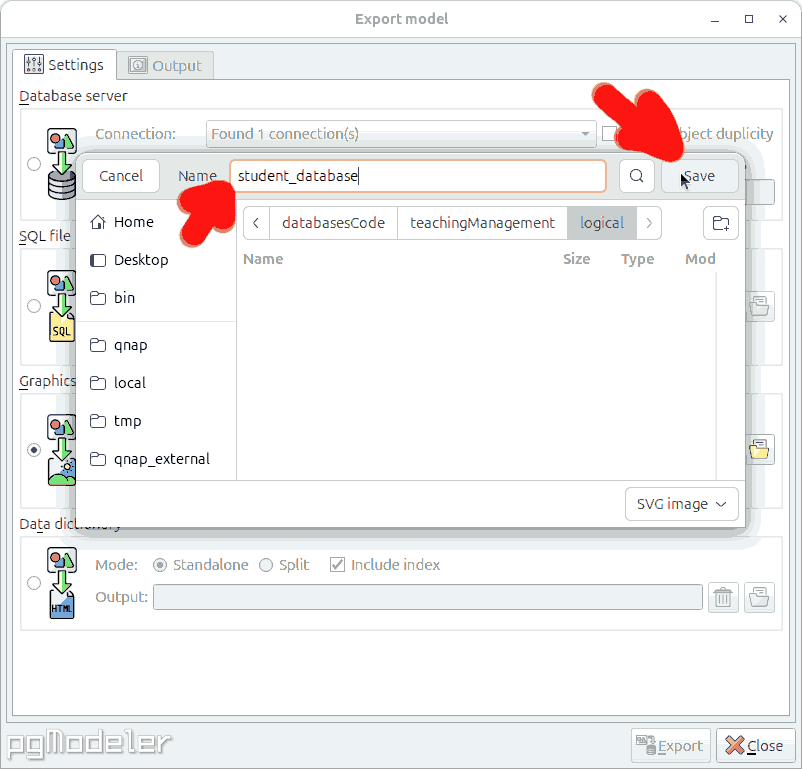
\includegraphics[width=0.48\linewidth]{\currentDir/makeStudentTable42fileName}}}%
%
\floatSep%
%
\subfloat[][%
We can now click on~\menu{Export}.%
\label{fig:makeStudentTable43exportToSvgExport}%
]{\tightbox{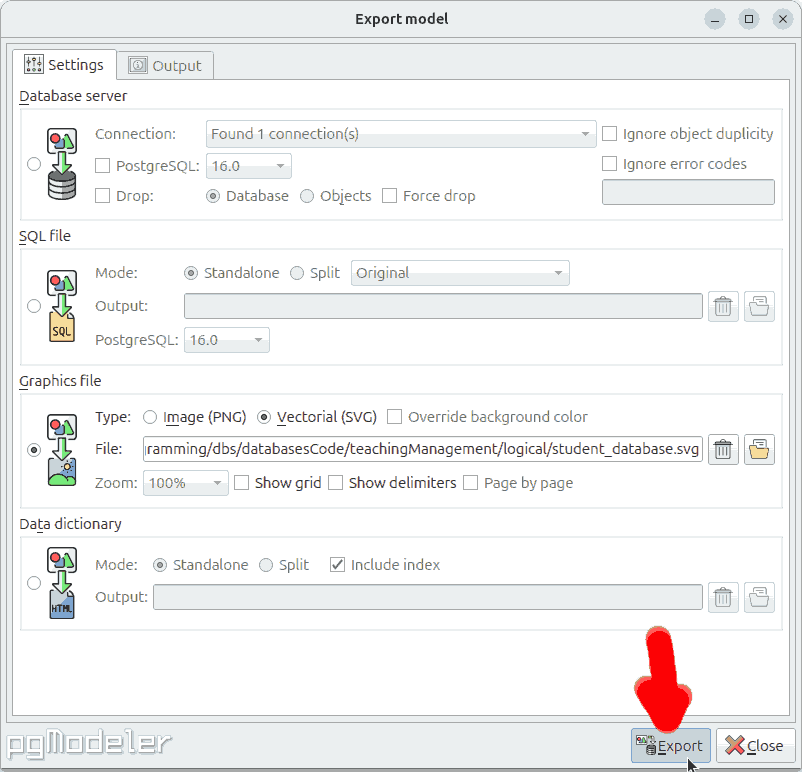
\includegraphics[width=0.48\linewidth]{\currentDir/makeStudentTable43exportToSvgExport}}}%
%
\floatRowSep%
%
\subfloat[][%
The file has been exported, we can close the dialog.%
\label{fig:makeStudentTable44exportToSvgExported}%
]{\tightbox{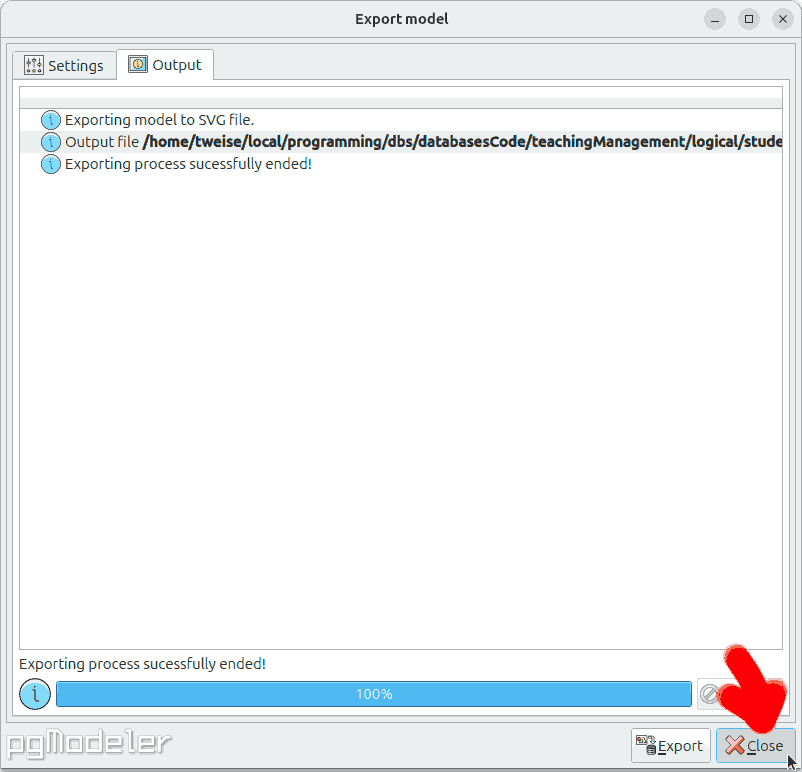
\includegraphics[width=0.48\linewidth]{\currentDir/makeStudentTable44exportToSvgExported}}}%
%
\floatSep%
%
\subfloat[][%
This is the exported vector graphic. %
It looks quite nice. %
If we had done a bigger model with many tables, it would probably look quite exciting.%
\label{fig:makeStudentTable45svg}%
]{\parbox[t]{0.48\linewidth}{\centering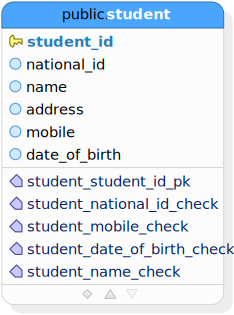
\includegraphics[width=0.66\linewidth]{\currentDir/makeStudentTable45svg}}}%
%
\label{fig:makeStudentTable:K}%
\caption{Developing logical models using \pgmodeler~(continued).}%
\end{figure}%
%
\begin{figure}%
\ContinuedFloat%
\centering%
%
\subfloat[][%
We open the \menu{Export} dialog again. %
This time, we want to export our model to~\sql. %
So we click on~\menu{SQL file} and then on the file bar.%
\label{fig:makeStudentTable46exportToSql}%
]{\tightbox{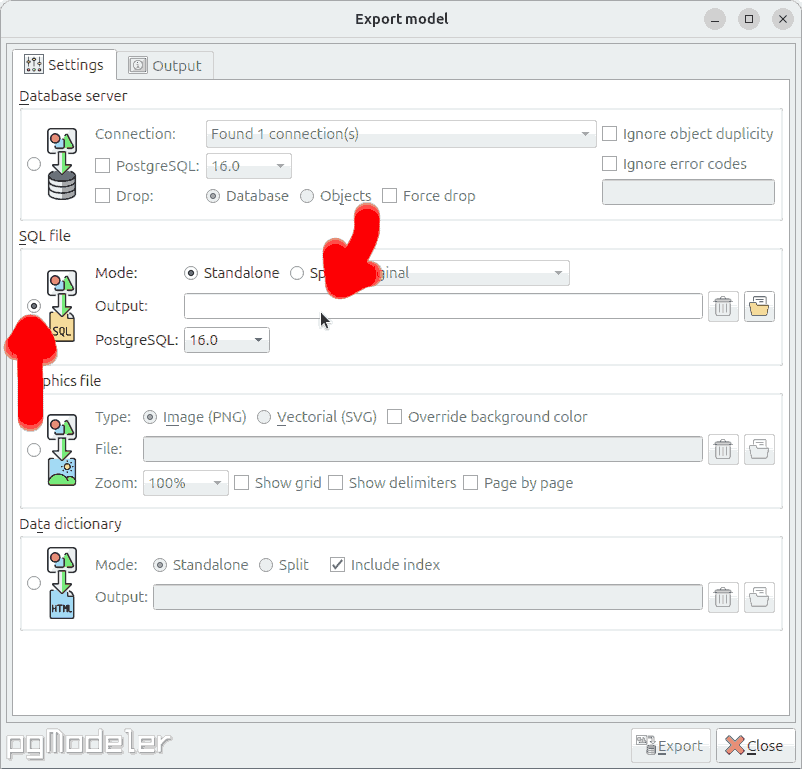
\includegraphics[width=0.48\linewidth]{\currentDir/makeStudentTable46exportToSql}}}%
%
\floatSep%
%
\subfloat[][%
As file name, we choose~\sqlil{student_database}. %
We click on~\menu{Save}.%
\label{fig:makeStudentTable47filename}%
]{\tightbox{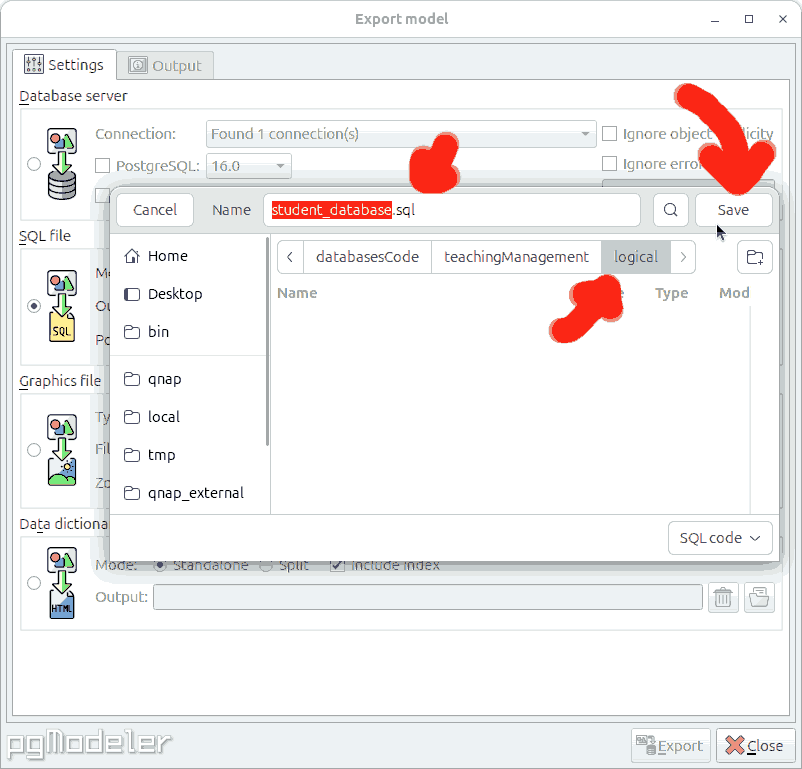
\includegraphics[width=0.48\linewidth]{\currentDir/makeStudentTable47filename}}}%
%
\floatRowSep%
%
\subfloat[][%
This takes us back to the dialog where we click on~\menu{Export}.%
\label{fig:makeStudentTable48exportToSqlExport}%
]{\tightbox{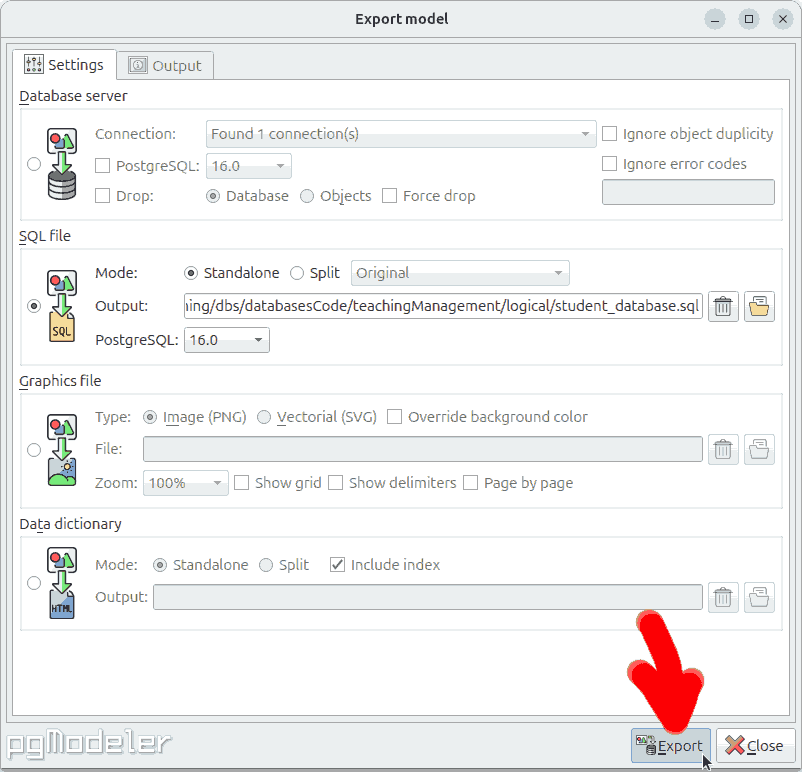
\includegraphics[width=0.48\linewidth]{\currentDir/makeStudentTable48exportToSqlExport}}}%
%
\floatSep%
%
\subfloat[][%
The model is exported and we close the dialog. %
We can now connect to the \postgresql\ \pgls{server} using \psql\ and execute the \sql\ commands that were exported. %
The exported commands are shown in \cref{lst:logical:teachingManagment:student_database}. %
If they are submitted to \psql, the output in \cref{exec:logical:teachingManagment:student_database} is created.%
\label{fig:makeStudentTable49exportToSqlExported}%
]{\tightbox{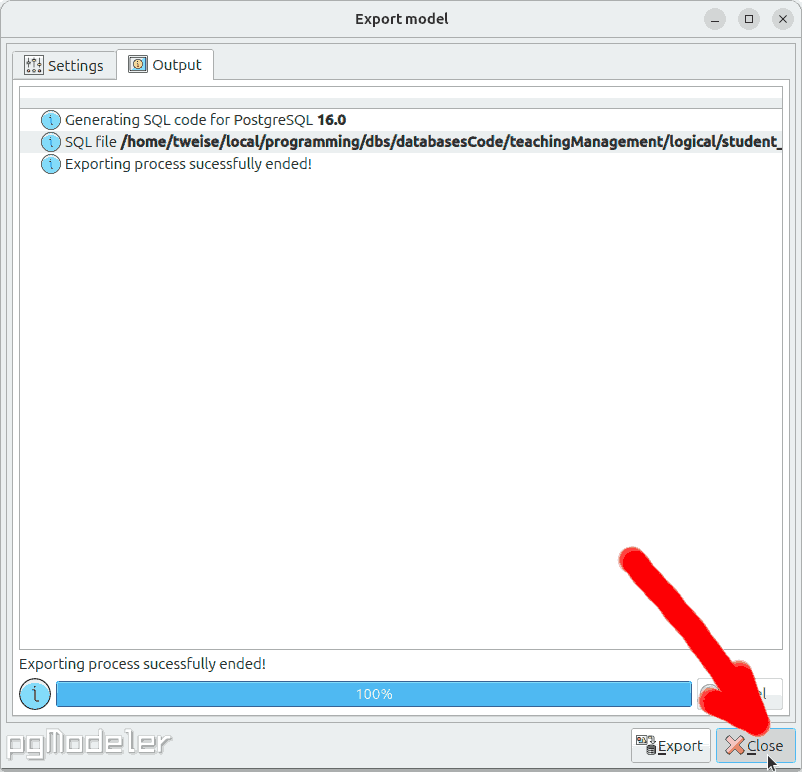
\includegraphics[width=0.48\linewidth]{\currentDir/makeStudentTable49exportToSqlExported}}}%
%
\label{fig:makeStudentTable:L}%
\caption{Developing logical models using \pgmodeler~(continued).}%
\end{figure}%
%
\gitSQLAndOutput{\databasesCodeRepo}{teachingManagement/logical}{student_database.sql}{}{}{}{postgres.sh}{logical:teachingManagment:student_database}{%
Executing the \sql\ script generated in \cref{fig:makeStudentTable48exportToSqlExport} on the \postgresql\ server. %
The \sqlil{student_database}, consisting of only a single table name~\sqlil{student}, is created.%
}%
%
\gitSQLAndOutput{\databasesCodeRepo}{teachingManagement/logical}{cleanup_student_database.sql}{}{}{}{postgres.sh}{logical:teachingManagement:student_database:cleanup}{%
Cleaning up after the student database example.%
}%
%
%
Back when we just began discussing conceptual models, we tried to model the entity type~\emph{Student}.
We drew an \pgls{ERD} for students as~\cref{fig:yedErdEntitiesA21erd}, which I here reproduce as \cref{fig:yedErdEntitiesA21erd2}.
Here, each entity of type \emph{Student} will have a name, an~ID, a student\nobreakdashes-ID, an address, a mobile phone number, and a \glsreset{dateOfBirth}\pgls{dateOfBirth}.
Later on, we realized that this model has many shortcomings and is not suitable for our teaching management platform.
Yet, it is fairly simple and suitable as an example for translating a single entity type from the conceptual model to the logical model.

We want to use the \pgmodeler\ for doing so.
Under \ubuntu\ \linux, we can start this program by opening a \pgls{terminal} by hitting \ubuntuTerminal, typing in \bashil{pgmodler}, and hitting~\keys{\enter}, as shown in \cref{fig:makeStudentTable01startPgmodeler}.
Under \microsoftWindows, you would instead proceed as shown in \cref{fig:installingPgModelerWindows22pgmodelerLogo}.

In the opened \pgmodeler\ window, we click on \menu{New Model} in \cref{fig:makeStudentTable02newModel}.
An empty \pgls{ERD} opens that represents an (empty) \db.
In a first step, we should choose a proper name for our \db.
We right-click at some place in the empty \pgls{ERD}.
In the context menu that opens up, we click on~\menu{Properties}, as shown in \cref{fig:makeStudentTable03rightClickProperties}.
A dialog called \inQuotes{Database Properties} opens.
As said, we want to set a proper name for our new \db.
We choose \sqlil{student_database} -- because the \db\ will only have a single table named \sqlil{student} -- and then click on~\menu{Apply} in \cref{fig:makeStudentTable04propertiesNameApply}.

Back in the \pgls{ERD} view it is now time for creating the table that will represent our \emph{Student} entity type.
We therefore again right-click into the (empty) diagram.
In the popup-menu, we click on~\menu{New>Schema Object>Table}, as illustrated in \cref{fig:makeStudentTable05newTable}.

The \inQuotes{Table properties} dialog opens in \cref{fig:makeStudentTable06tableNameColumns}.
We can choose a table name and, as said, we pick \sqlil{student} and type this in.
The attributes of an entity type become attributes in a relation in a relational logical schema, which are embodied as columns of a table.
To add such columns, we click on the register~\menu{Columns}.
The columns register is still empty.
We click on the \menu{Add Item} symbol~\pgmodelerAddItem\ in \cref{fig:makeStudentTable07newColumn}.

In a first step, we want to create a column for the university-issued student~ID.
As name for this column, we choose~\sqlil{student_id}.
This is better than using~\sqlil{ID}, because it conveys a clear meaning that this is, in fact, the student~ID.
Everybody will immediately understand what this means.
Student~IDs are usually strings of a fixed length.
We therefore choose the \menu{Type}~\sqlil{character}\sqlIdx{CHARACTER} in \cref{fig:makeStudentTable08studentIdNameAndType}.
In \sql, this is the datatype for fixed-length strings.
As (fixed) length, we enter~11 in the \menu{L:}~field.
This means that all student~IDs that we store in our \db\ will be text strings consisting of eleven characters.
We also mark the column as \sqlilIdx{NOT NULL}.
This means that there cannot be a student record where the \sqlil{student_id} is \sqlilIdx{NULL}.
This, in turn, means that there cannot be a student record without student~ID.
\sqlil{student_id} is a mandatory field that always needs to be provided.
In \cref{fig:makeStudentTable09studentIdLenNotNullApply}, we click~\menu{Apply}.%
%
\bestPractice{columnNames}{%
To avoid issues with quotations, it is best to use only lower case character names and underscores~(\sqlil{_}) to separate nouns for all named things in \pgmodeler, including tables, columns, and constraints.%
}%
%
The new column appears in the table creation dialog.
We now want to add the next column, so we click again on~\menu{Add Item}~\pgmodelerAddItem\ in \cref{fig:makeStudentTable10studentIdAddedNewColumn}.
The next important piece of data of each student record is a national Chinese~ID number~(中国公民身份号码).
We add the column \sqlil{national_id} for storing Chinese~ID numbers.
As per standard \mbox{GB11643\nobreakdashes-1999} \citetitle{GB116431999CIN}~\cite{GB116431999CIN}, such numbers always consist of 18~characters.
So we choose the atatype \sqlil{character}\sqlIdx{CHARACTER} with the fixed length~18.
We here ignore the fact that there could be foreign exchange students~(留学生) and demand that all records must have \sqlil{national_id} field set by marking the column as~\sqlilIdx{NOT NULL}.
We click~\menu{Apply} in \cref{fig:makeStudentTable11nationalIdNameTypeLenNotNullApply}.

The new column appears in \cref{fig:makeStudentTable12nationalIdAddedNewColumn} and we click~\menu{Add Item}~\pgmodelerAddItem.
We now define the column \sqlil{name} for student names.
Names are text strings of variable length, which corresponds to the \sql\ datatype \sqlil{varchar}\sqlIdx{VARCHAR}.
We set the \emph{maximum} length to 255~characters, which is fairly large and should be long enough for most sensible names.
Each student must have a name, so we again specify \sqlil{NOT NULL} and click~\menu{Apply} in \cref{fig:makeStudentTable13nameNameTypeLenNotNullApply}.

The new column appears in \cref{fig:makeStudentTable14nameAddedNewColumn} and we click again on~\menu{Add Item}~\pgmodelerAddItem.
The next column we want to add is for storing the addresses of the students.
We call this column \sqlil{address}.
Here, we again use strings of variable length~(type \sqlil{varchar}\sqlIdx{VARCHAR}) as datatype.
We again set the maximum length to 255~characters.
We also again require the field to be \sqlilIdx{NOT NULL} and click~\menu{Apply} in \cref{fig:makeStudentTable15addressNameTypeLenNotNullApply}.

The new column appears in \cref{fig:makeStudentTable16addressAddedNewColumn} and we click~\menu{Add Item}~\pgmodelerAddItem.
We now add a column for \sqlil{mobile} phone numbers.
Mobile phone numbers in China have 11~digits~\cite{BD2006BDBK:MPNANSBTTMDFMP}.
We can thus store them as strings~~(\sqlil{character}\sqlIdx{CHARACTER}) of the fixed length~11.
We require that they must be specified~(\sqlilIdx{NOT NULL}) and click~\menu{Apply} in \cref{fig:makeStudentTable17mobileNameTypeLenNotNullApply}.

The new column appears in the table dialog and we again click on~\menu{Add Item}~\pgmodelerAddItem\ in \cref{fig:makeStudentTable18mobileAddedNewColumn}.
Finally, we add the \pgls{dateOfBirth} in form of the \sqlil{date_of_birth} column.
The datatype here is \sqlil{date}\sqlIdx{DATE}.
Like all the columns so far, we require that \pglspl{dateOfBirth} to be \sqlilIdx{NOT NULL}.
We click~\menu{Apply} in \cref{fig:makeStudentTable19dateOfBirthNameTypeNotNullApply}.

The new column appears in~\cref{fig:makeStudentTable20dateOfBirthAddedConstraints}.
In the above text, you may have noticed that we are quite lenient with the data.
For example, mobile phone numbers are not strings of arbitrary characters, but consist only of digits.
Chinese ID~numbers also are composed of digits, with the exception that the last character might be an~\textil{X}.
Also, we should probably not permit arbitrary dates as \pglspl{dateOfBirth}.
Even though September~23,~1811 would be a totally valid date, as the \pgls{dateOfBirth} of a student it would be unusual.
Actually, we already learned how to deal with such restrictions on valid data back in \cref{sec:factory:table:customer}:
by using constraints.
We also did not yet define a primary key~(see \cref{sec:primaryKey}) for our table.

We click on the register \menu{Constraints}, because now we want to add validity rules for our data.
In the \menu{Constraints} register, we click~\menu{Add Item}~\pgmodelerAddItem, as shown in \cref{fig:makeStudentTable21newConstraint}.
If you think about, we can consider the fact that a column is the \emph{primary key} as a combination of a \sqlilIdx{UNIQUE} and a \sqlilIdx{NOT NULL} constraint~(maybe together with some special indexing for fast access).
So first, we want to choose a primary key.

What would be the most suitable column?
The columns \sqlil{name}, \sqlil{address}, and \sqlil{date_of_birth} are unsuitable -- if not for obvious reasons -- then at least because they are not necessarily unique.
The two columns \sqlil{student_id} and \sqlil{national_id} both look promising a primary keys.
However, a person may enroll several times, maybe first as Bachelor and later as Master's student.
Hence, \sqlil{national_id} is not necessarily unique.
But for each enrollment, the person gets a new \sqlil{student_id}, which therefore is unique.
As first constraint, we thus want to define \sqlil{student_id} as the primary key of our table.

We call this constraint \sqlil{student_student_id_pk} and select \sqlilIdx{PRIMARY KEY} as type.
We select the column \sqlil{student_id} in the \menu{Column} drop-down box and click on~\menu{Add Item}~\pgmodelerAddItem\ in \cref{fig:makeStudentTable22studentIdPkData}.
The column \sqlil{student_id} appears in the \menu{Columns} list.
We click on~\menu{Apply} in \cref{fig:makeStudentTable23studentIdColAddedApply}.%
%
\bestPractice{constraintNames}{%
Constraints should have descriptive names~\cite{B2025DS:SBPASG}. %
If some table modification fails, we will see the name of the constraint that was violated. %
If the name makes sense and is easy to understand, then this makes it easier to find out what went wrong and why.%
}%
The new constraint appears and we click on \menu{Add Item}~\pgmodelerAddItem\ in \cref{fig:makeStudentTable24studentIdAddedNewConstraint}.
We now want to add a constraint checking that the national~ID is correct.
We call it \sqlil{student_national_id_check} and select \sqlil{CHECK}\sqlIdx{CONSTRAINT!CHECK} in the \menu{Type} drop-down box in \cref{fig:makeStudentTable25nationalIdCheck}.
Indeed, we are going to create a \sqlil{CHECK} constraint\sqlIdx{CONSTRAINT!CHECK}.
For this, we just need to provide an \sql\ \menu{Expression}.
This expression is evaluated whenever a row is added to the table or when a row is changed.
If it then returns~\sqlil{TRUE}, everything is fine.
If it returns~\sqlil{FALSE}, then the change will not be made.

So back to the Chinese~ID numbers~(中国公民身份号码).
How do we check them?
Standard \mbox{GB11643\nobreakdashes-1999} \citetitle{GB116431999CIN}~\cite{GB116431999CIN} tells us that the first six digits are the administrative division code.
The next eight digits are the \pgls{dateOfBirth} in format YYYYMMDD, followed by three digits of order code.
The last character is a single checksum digit~(which can be~X).
We could check this in a super fancy fashion.
We could get our hands on a list of the actual valid values for the first digits, assuming that not all possible 999'999~possible administrative division codes are actually valid.
We could compare the next six digits to the \pgls{dateOfBirth} that we store as well\footnote{%
On second thought, if we require ID numbers to be present, we would not need to store the \pgls{dateOfBirth} anymore {\dots} but well, now we did it and will stick to it.}.
We could even try to compute the checksum digit and check whether it matches.

This is all too complicated for us.
Instead, we will resort to a \glsreset{regex}\pgls{regex} to check the field like back in \cref{sec:factory:table:customer}.
We write \expandafter\sqlil{national_id ~ '^\\d\{6\}((19)|(20))\\d\{9\}[0-9X]\$'}.
The \sqlil{national_id ~ xxx} means that the value of \sqlil{national_id} must match to some \pgls{regex}~\textil{xxx}.
In the \pgls{regex}, \textil{^}~indicates the start of the text.
\textil{\\d\{6\}}~means that six digits must immediately follow~\textil{^}, i.e., be right at the start of the string.
Then comes \textil{((19)|(20))}, which means that the next two characters must be either \inQuotes{19} or \inQuotes{20}.
This is because we do not permit \pglspl{dateOfBirth} before the year 19\textcolor{gray}{00} or after 20\textcolor{gray}{99}.
After that, we require nine digits to follow via~\textil{\\d\{9\}}.
This means we now have $6+2+9=17$~digits, leaving the final checksum character, which can be any digit from 0~to~9 or~X.
This is expressed by the~\textil{[0-9X]}.
The~textil{\$} that follows marks the end of the string, which, hence, must come directly after the checksum digit.

We click~\menu{Apply} in \cref{fig:makeStudentTable26nationalIdConstraintApply} and the constraint is specified.
The new constraint appears and we click on~\menu{Add Item}~\pgmodelerAddItem\ in \cref{fig:makeStudentTable27nationalIdAddedNewConstraint}.

We now create a similar \sqlil{CHECK}\sqlIdx{CONSTRAINT!CHECK}~constraint for the column~\sqlil{mobile} in \cref{fig:makeStudentTable28mobileCheck}.
We call it~\sqlil{student_mobile_check}.
The expression~\sqlil{mobile ~ '^\\d\{11\}\$'} demands an 11~digit string:
It states that the \sqlil{mobile} value must, right at its begin~(\textil{^}), have eleven digits~(\textil{\\d\{11\}}), and then the end of the string follows immediately~(\textil{\$}).
We click on~\menu{Apply}.

The new constraint appears and we click on~\menu{Add Item}~\pgmodelerAddItem\ again in \cref{fig:makeStudentTable29mobileAddedNewConstraint}.
We want to specify the \sqlil{CHECK}\sqlIdx{CONSTRAINT!CHECK} constraint for the \pgls{dateOfBirth} and call it~\sqlil{student_date_of_birth_check}.
We combine the condition \sqlil{date_of_birth > '1900-01-01'} (demanding that students may not be born before the year~1900) and \sqlil{date_of_birth < '2100-01-01'}~(which prevents students born in the 22nd century) with~\sqlilIdx{AND}.
We click~\menu{Apply} in \cref{fig:makeStudentTable30dateOfBirthCheck}.

In \cref{fig:makeStudentTable31dateOfBirthAddedNewConstraint}, the new constraint appears and we click on~\menu{Add Item}~\pgmodelerAddItem.
As final constraint, we want to set some restriction on valid names.
We create a \sqlil{CHECK}\sqlIdx{CONSTRAINT!CHECK}~constraint for the column~\sqlil{name} and call it~\sqlil{student_name_check}.
We specify the expression~\expandafter\sqlil{name ~ '^\\S+.*\\S+\$'}.
The \textil{\\S} matches a single character that is not whitespace, i.e., a character that is neither space nor a line break nor a tabulator.
The \textil{+} means \inQuotes{one or multiple repetitions of the previous}, so \textil{\\S+} means \inQuotes{one or multiple non-space characters}.
We want the name to start (and end) with a letter or Chinese character or maybe Indian character or whatever, but no reasonable name starts with a space.
We force such a non-space character to be at the beginning~(\textil{^\\S+}) and at the end~(\textil{\\S+\$}) of the string~\sqlil{name}\footnote{%
On second thought, we could have left the \textil{+}s away.%
}. %
Inbetween, we permit an arbitrary number~(\textil{*}) of arbitrary characters~(\textil{.}).
Thus, this expression  demands that names both start and end with printable characters and may contain an arbitrary number of characters in between
We click on~\menu{Apply} in \cref{fig:makeStudentTable32nameCheck}.

The new constraint appears.
We stop here.
Yes, we could add a similar constraint for the columns \sqlil{address}.
And indeed, we did not match the \pgls{dateOfBirth} stored as \sqlil{date_of_birth} in the table against the \pglspl{dateOfBirth} encoded in the field~\sqlil{national_id}.
We also did not impose a constraint upon the \sqlil{student_id}, except that these values have to be \sqlilIdx{UNIQUE} and \sqlilIdx{NOT NULL}.
Well, for this simple example, I think we are good.
We now create the table model by clicking on~\menu{Apply} in \cref{fig:makeStudentTable33nameCheckAddedApply}.

The new table appears in our \pgls{ERD}, with a syntax similar to what we had in \cref{sec:compactCrowsFootNotation}.
It is now time to save this logical model to a file.
We click on~\menu{\pgmodelerMainMenu>File>Save as} in \cref{fig:makeStudentTable35saveAs}.
Since our model is new and unchecked (or changed), we get asked to validate it.
This seems to be a reasonable request and we click on~\menu{Validate} in \cref{fig:makeStudentTable36shouldValidate}.
Next we can select a file name and directory where the model should be stored.
We choose the name \sqlil{student_database} and click~\menu{Save} in \cref{fig:makeStudentTable37saveAsWhere}.

This takes us back to the main window.
We notice a bar with new buttons, including one called~\menu{Validate}.
This must be the meaning of the request to validate our model in \cref{fig:makeStudentTable36shouldValidate}.
So now we click on it in \cref{fig:makeStudentTable38validate}.
Our model gets validated.
It is OK.
We can close the log in \cref{fig:makeStudentTable39validated}.

So far, however, we did not really do anything useful with this logical model.
When we used \yEd\ to draw our conceptual model, we could export it as \glsreset{SVG}\pgls{SVG} graphic.
We can also do this with models created in the \pgmodeler.
We therefore click on~\menu{Export} in \cref{fig:makeStudentTable40export}.

We want to store the model as \pgls{SVG} graphic.
Therefore, we click on \menu{Graphics file} and select \menu{Vectorial~(SVG)}.
We then click into the \menu{File}~bar in \cref{fig:makeStudentTable41exportAsSvg}.
We again get to select a file name and again stick with \sqlil{student_database}.
In \cref{fig:makeStudentTable42fileName}, we click on~\menu{Save}.
This takes us back to the export dialog in \cref{fig:makeStudentTable43exportToSvgExport}.
Here we can now click on~\menu{Export}.
The file has been exported, we can close the dialog in \cref{fig:makeStudentTable44exportToSvgExported}.

In \cref{fig:makeStudentTable45svg}, we illustrate the exported vector graphic.
It looks quite nice.
If we had done a bigger model with many tables, it would probably look quite exciting.

This is the extend of what we could do on the conceptual modelling level, too.
There, we could paint a model and print it as graphic.
We also painted a model now.
The logical model we did paint had a much tighter syntax is a formal model.
We used specific \sql\ datatypes, \sql\ constraints, and could do nothing that cannot be done with \sql.
In stark contrast, \yEd\ allows us to paint almost arbitrary graphics.
We could have drawn stars and clouds into our \pgls{ERD} if we wanted to.

However, sticking to \sql\ (or, more precisely, the \postgresql\ flavor of it), has another advantage:
We can actually create a \db\ from our model!

We therefore open the \menu{Export} dialog again.
This time, we want to export our model to~\sql.
So we click on~\menu{SQL file} and then on the file bar in \cref{fig:makeStudentTable46exportToSql}.
As file name, we choose~\sqlil{student_database}.
In \cref{fig:makeStudentTable47filename}, we click on~\menu{Save}.
This takes us back to the export dialog where we click on~\menu{Export} in \cref{fig:makeStudentTable48exportToSqlExport}.

The model is exported and we close the dialog in~\cref{fig:makeStudentTable49exportToSqlExported}.
\Cref{lst:logical:teachingManagment:student_database} shows the file \textil{student_database.sql} which was created from our logical model.
This, indeed, is \sql\ -- not different from what we produced manually in the context of our simple factory example in \cref{sec:factoryCreatingTableAndInsertingData}.

We can now connect to the \postgresql\ \pgls{server} using \psql\ and execute the \sql\ commands that were exported.
If \cref{lst:logical:teachingManagment:student_database} is submitted to \psql, the output in \cref{exec:logical:teachingManagment:student_database} is produced.
It works!
The \db\ and the table are created exactly as expected.
What does this mean?
It means the following:%
%
\usefulTool{pgmodeler}{%
With \pgmodeler, we have a tool in our hands that allows us to basically draw logical models for \pglspl{db} as \pglspl{ERD}. %
These models are easy-to-understand graphics that follow crow's foot notation. %
\pgmodeler\ can connect to a \postgresql\ \pgls{server} and directly push the models to it or load a logical model from the \pgls{server}. %
It can also export logical models as \sql\ scripts that we then can execute.
It therefore offers us a convenient \pgls{GUI} to design the logical schema of a \db.%
}%
%
Of course, \pgmodeler\ is not the only such software.
But it is quite nice, open source, and free.
It is suitable for \postgresql, while other programs have been developed for other \pglspl{dbms}.
As said in \cref{bp:manyTools}, good software engineers are both able and keen to learn new tools.

To depart from this example with a clean slate, we execute the \sql\ script given in \cref{lst:logical:teachingManagement:student_database:cleanup} to delete the table and \db\ again.%
%
\FloatBarrier%
\endhsection%
%
